%==============================================================================    
\chapter{Pixel chip electronics and calibration}
\label{ch:FE_electronics}
%==============================================================================    

One of the key components of the detector systems is the readout
electronics. Each experiment, depending on the requirements, has its
own specific electronics. But the basic principles of the electronics
and optimisations of the signal-to-noise remain similar between
different applications.

In this chapter, we will review the basic principles and requirements
of a readout chip. The Timepix readout chip families are described in
the following sections since they are used to study thin and
active-edge assemblies in the following chapters. They are calibrated
using different methods and the MIP energy deposition measured by
these chips is compared to \textsc{Geant4} simulations.

\section{Generic pixel chip properties}

The main purpose of the detecting system is to acquire the signal
generated in the sensor which is in the form of a short current
pulse. The electronics are responsible for shaping the time response
of the system in order to optimise the minimum detectable signal,
energy deposition in detector measurement, event rate, time-of-arrival
and insensitivity to the pulse shape. Finally, the signal is digitised
and stored. Robustness to radiation and power consumption are other
important considerations to be addressed amongst others.

\cref{fig:detectorFunctions} schematically overviews the basic
detector functions. The incident radiation deposits energy in the
sensor and it is converted to an electrical signal. A high rate of
particles can be handled in a semiconductor detector because the
sensor pulse is very short (few nanoseconds). Since the magnitude of
the signal charge can be small and is subject to statistical
fluctuations (\cref{sec:chargeInSi}), a preamplifier is needed to
amplify the signal. The preamplifier should be designed in such a way
to minimise the electronic noise. The sensor capacitance and the input
capacitance of the amplifier are the critical parameters to increase
the signal-to-noise ratio (SNR): the lower the capacitance, the higher
the SNR. After the preamplifier, the pulse shaper is responsible for the
improvement of the SNR. It modifies the frequency response of the
signal to improve the signal and attenuate the noise. Since this
operation reduces the bandwidth of the signal, the duration of the
pulse will increase. A detector must cope with a high rate of pulses,
the width of the pulse must be optimised in a way to reduce the
pile-up.

The analog-to-digital converter (ADC) converts a continuously varying
amplitude to discrete steps. When the pulse height passes a threshold
in a comparator, counters are incremented to measure the energy and
the timing of the signal for example.

\begin{figure}[htbp]
  \centering
  \begin{tikzpicture}
      \begin{scope}[x={(image.south east)},y={(image.north west)}]
        % \draw[help lines,xstep=.1,ystep=.1] (0, 0) grid (1,1);
        % \foreach \x in {0,1,...,9} { \node [anchor=north] at (\x/10,0) {0.\x}; }
        % \foreach \y in {0,1,...,9} { \node [anchor=east] at (0,\y/10)
        %   {0.\y}; }

        %\path (-0.1, 0.5) -- ++(0.08, 0.5) node[rv] {Incident radiation};
        \draw (0.1, 0.4) rectangle (0.3, 0.6) node[pos=.5] {Sensor};
        \draw (0.4, 0.6) -- (0.4, 0.4) -- (0.6, 0.5) -- cycle;
        \node[above] at (0.5, 0.65) {Preamplifier};
        \draw (0.7, 0.6) -- (0.7, 0.4) -- (0.9, 0.5) -- cycle;
        \node[above] at (0.8, 0.65) {Pulse shaping};
        \draw (1, 0.35) rectangle (1.3, 0.65) node[pos=.5] {ADC converter};
        % \node[above] at (1.15, 0.7) {Analog to digital convertor};

        \draw[arrows=->](-0.1, 0.5)--(0.08, 0.5) node [pos=0.1, above]
        {Incident radiation};

        \draw[arrows=->](0.3, 0.5)--(0.4, 0.5);
        \draw[arrows=->](0.6, 0.5)--(0.7, 0.5);
        \draw[arrows=->](0.9, 0.5)--(1, 0.5);
        \draw[arrows=->](1.3, 0.5)--(1.5, 0.5) node [pos=0.8, above]
        {Digital data bus};
        

      \end{scope}
  \end{tikzpicture}
  \caption{Schematic overview of basic detector functions.}  
  \label{fig:detectorFunctions}
\end{figure}

\cref{fig:TOT_TOA_concept} schematically shows the energy and the
timing measurement of the signal. The Time-over-threshold (TOT) allows
for the measurement of the energy deposited in a pixel. The pulse is
amplified and the pulse shaper integrates the signal to form a step
pulse with a long linear decay. The decay is approximately linear and
proportional to the energy deposited. While the pulse is above the
programmable threshold, the counter is incremented.

The Time-of-Arrival (TOA) measures the arrival time of a hit and
therefore is used as a time stamping of the hits. When the amplifier
output exceeds the pixel threshold, the discriminator output rises and
the fast TOA (FTOA) counter counts until the rising edge of the
general clock. A combination of the TOA and the FTOA counters is used
as the timing information for the hits.

\begin{figure}[htbp]
  \centering
  \begin{tikzpicture}
    \begin{scope}[x={(image.south east)},y={(image.north west)}]
      % \draw[help lines,xstep=.1,ystep=.1] (0, 0) grid (1,1);
      % \foreach \x in {0,1,...,9} { \node [anchor=north] at (\x/10,0) {0.\x}; }
      % \foreach \y in {0,1,...,9} { \node [anchor=east] at (0,\y/10)
      % {0.\y}; }
      
      % pulse
      \draw[-, thick] (0.1, 0.8) -- (0.2, 0.8);
      \draw[-, thick] (0.2, 0.8) -- (0.21, 0.98);
      \draw[-, thick] (0.21, 0.98) -- (0.22, 0.8);
      \draw[-, thick] (0.22, 0.8) -- (1, 0.8);

      % shaper
      \draw[-, thick] (0.1, 0.5) -- (0.2, 0.5);
      \draw[-, thick] (0.2, 0.5) -- (0.22, 0.7);
      \draw[-, thick] (0.22, 0.7) -- (0.8, 0.5);
      \draw[-, thick, dashed, green] (0.1, 0.55) -- (0.8, 0.55);
      \draw[-, thick] (0.8, 0.5) -- (1, 0.5);

      % comparator
      \draw[-, thick] (0.1, 0.3) -- (0.21, 0.3);
      \draw[-, thick] (0.21, 0.3) -- (0.21, 0.4);
      \draw[-, thick] (0.21, 0.4) -- (0.65, 0.4);
      \draw[-, thick] (0.65, 0.4) -- (0.65, 0.3);
      \draw[-, thick] (0.65, 0.3) -- (1, 0.3);

      \timing [] at (0.1,0.2) {LLLHHLLHHLLHHLLHHLLHHLLLL};
      \draw[arrows=<->, thick](0.21, 0.15)--(0.65, 0.15) node [pos=0.5, below]
      {\textbf{TOT (3 counts)}};

      \timing [] at (0.1,0.0) {llllllhlhlhlhllllllllllllllllllllllllllllllllllllll};

      \draw[-, thick, dashed, blue] (0.21, 0.55) -- (0.21, 0.0);
      \draw[-, thick, dashed, blue] (0.65, 0.55) -- (0.65, 0.0);

      \draw[-, thick, dashed, red] (0.35, 0.2) -- (0.35, 0.0);

      \draw[arrows=<->, thick](0.21, -0.05)--(0.35, -0.05) node [pos=0.5, below]
      {\textbf{FTOA (4 counts)}};


      \node[left] at (0.1, 0.8) {Sensor pulse};
      \node[left, green] at (0.1, 0.6) {Threshold};
      \node[left] at (0.1, 0.5) {Pulse after shaping};
      \node[left] at (0.1, 0.3) {Discriminator output};
      \node[left] at (0.1, 0.2) {General clock}; %$40\,\megahertz$ Clk}
      \node[left] at (0.1, 0.0) {FTOA clock}; %$640\,\megahertz$ Clk (FTOA)     


    \end{scope}
  \end{tikzpicture}
  \caption{Schematic overview of the Time-over-Threshold (TOT) and
    Time-of-Arrival (TOA) measurements in a readout chip.}  
  \label{fig:TOT_TOA_concept}
\end{figure}

\section{The Timepix readout chip families}\label{sec:TimepixReadout}
The Timepix~\cite{art:tmpx,Timepix3Poikela} readout chip families,
designed by the Medipix collaboration, are a general purpose front-end
electronics and can measure precisely the energy deposited in the
sensor and also provide accurate timing information. An overview on
the Timepix and Timepix3~\cite{Timepix3Poikela} chip families is given
in~\cref{tab:timepixOverview}. They consist of $256\times256$ pixel
matrix with pixels pitch of $55\,\micron$. The both chip families
allow for three operation modes: photon counting, TOT and TOA
measurements. Timepix3 allows for simultaneous measurement of the TOT
and the TOA with a timing resolution of 1.6~ns.

\begin{table}[htbp]
  \centering
  \caption{Overview of Timepix readout ASICs.}
  \label{tab:timepixOverview}
  \begin{tabular}{l c c}
    \toprule
    & Timepix& Timepix3\\ 
    \midrule
    Pixel Matrix & $256\times256$ & $256\times256$\\
    Pixel Pitch [\micron] & 55 & 55\\
    Technology & $0.25\,\micron$ CMOS & 130~nm CMOS\\
    Counter Depth & 14 bits & 10 bit TOT and 18 bit TOA \\
    Readout Type & Frame based & Data driven \& frame based \\
    Electronic Noise & $\sim100$ e\textsuperscript{-} RMS & $<70$ e\textsuperscript{-} RMS\\
    \bottomrule
  \end{tabular}
\end{table}

\cref{fig:Timepix_pixel_cell_schematic} shows schematically the
functionalities implemented in a Timepix pixel cell. Both analogue and
digital circuitry are combined. The analogue circuitry includes a
charge sensitive amplifier with a tunable discharge current of the
Krummenacher amplifier architecture
(I\textsubscript{krum})~\cite{KRUMMENACHER1991527} and the
discriminator. I\textsubscript{krum} affects the slope of the pulse
discharge after shaping: the higher its value, the shorter the
pulse. The discriminator is used to compare the signal level to a
threshold (a voltage) and to discriminate a signal from a background
noise. Both polarities (electrons and holes collection) are accepted
by the front end.

The Timepix3 readout chip allows for a data driven readout mode which
can reach higher readout rates than the frame based mode. In the data
driven mode, after a hit is processed by the pixel, a data packet
containing the TOT and the TOA information is immediately sent off the
chip. This reduces significantly the dead time of the pixels and
allows to reach very high readout rates.

\begin{figure}[htbp] 
  \centering
  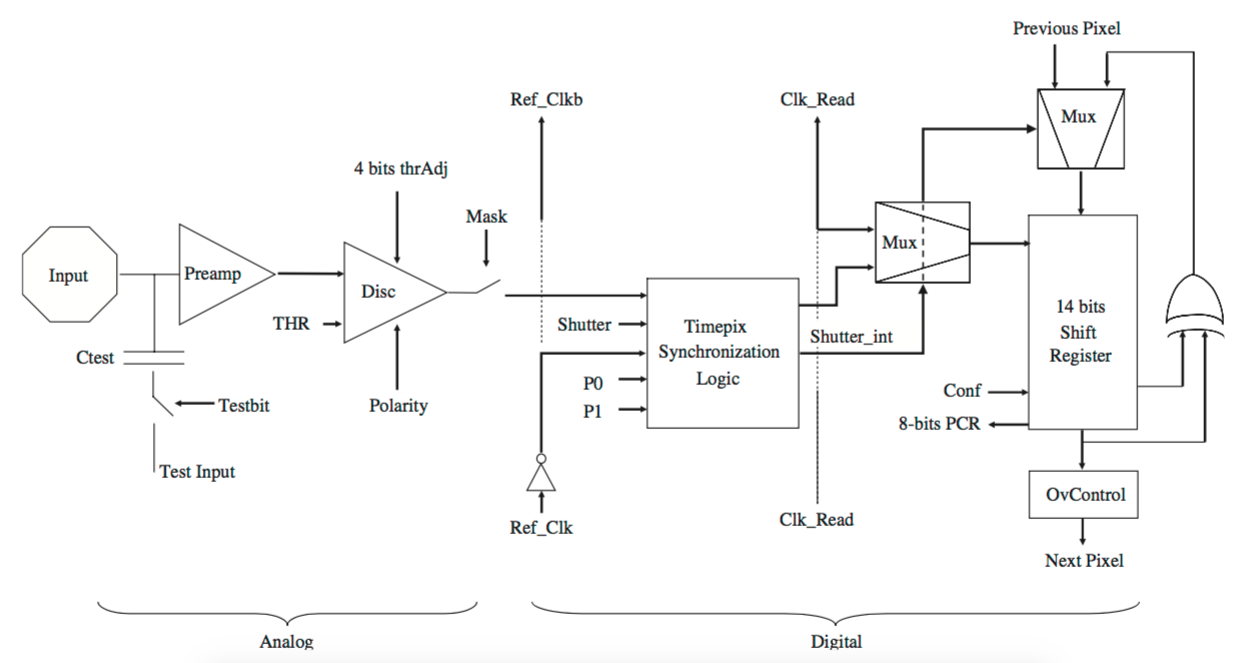
\includegraphics[width=\textwidth]{./figures/Calibration/Timepix_pixel_cell_schematic.jpg}
  \caption{Timepix pixel cell schematic. From ~\cite{art:tmpx}.}
  \label{fig:Timepix_pixel_cell_schematic}
\end{figure}

\subsection{Threshold equalisation} \label{sec:ThresholdEqualisation}
In semiconductor electronics, manufacturing imperfections cause
variations in the performance within the device. The threshold is one
of the most affected parameters and its global value set can vary
highly from one pixel to another within the pixel matrix. For the same
threshold value, the voltage on the discriminator can vary highly from
one pixel to another. To overcome this dispersion, a 4-bit local
threshold adjustment is applied to each pixel in order to make a
uniform global threshold. The photon counting mode is then
employed. The equalisation consists of adjusting this local threshold
by first setting its value to the mask 0000. The global threshold DAC
(Digital-to-Analog), THL, is scanned and the number of pixels
responding are counted. Then the adjustment bit is set to 1111 and THL
is scanned again. For each pixel, the operation range is
known. Assuming a linear relationship between the two points, the
adjustment threshold is adjusted in such a way that the global
threshold dispersion will remain uniform across the matrix.

\cref{fig:THLequalisation} shows the threshold equalisation for an
assembly. After equalisation the response of the chip becomes more
uniform even though some dispersion remains.

\begin{figure}[htbp] 
  \centering
  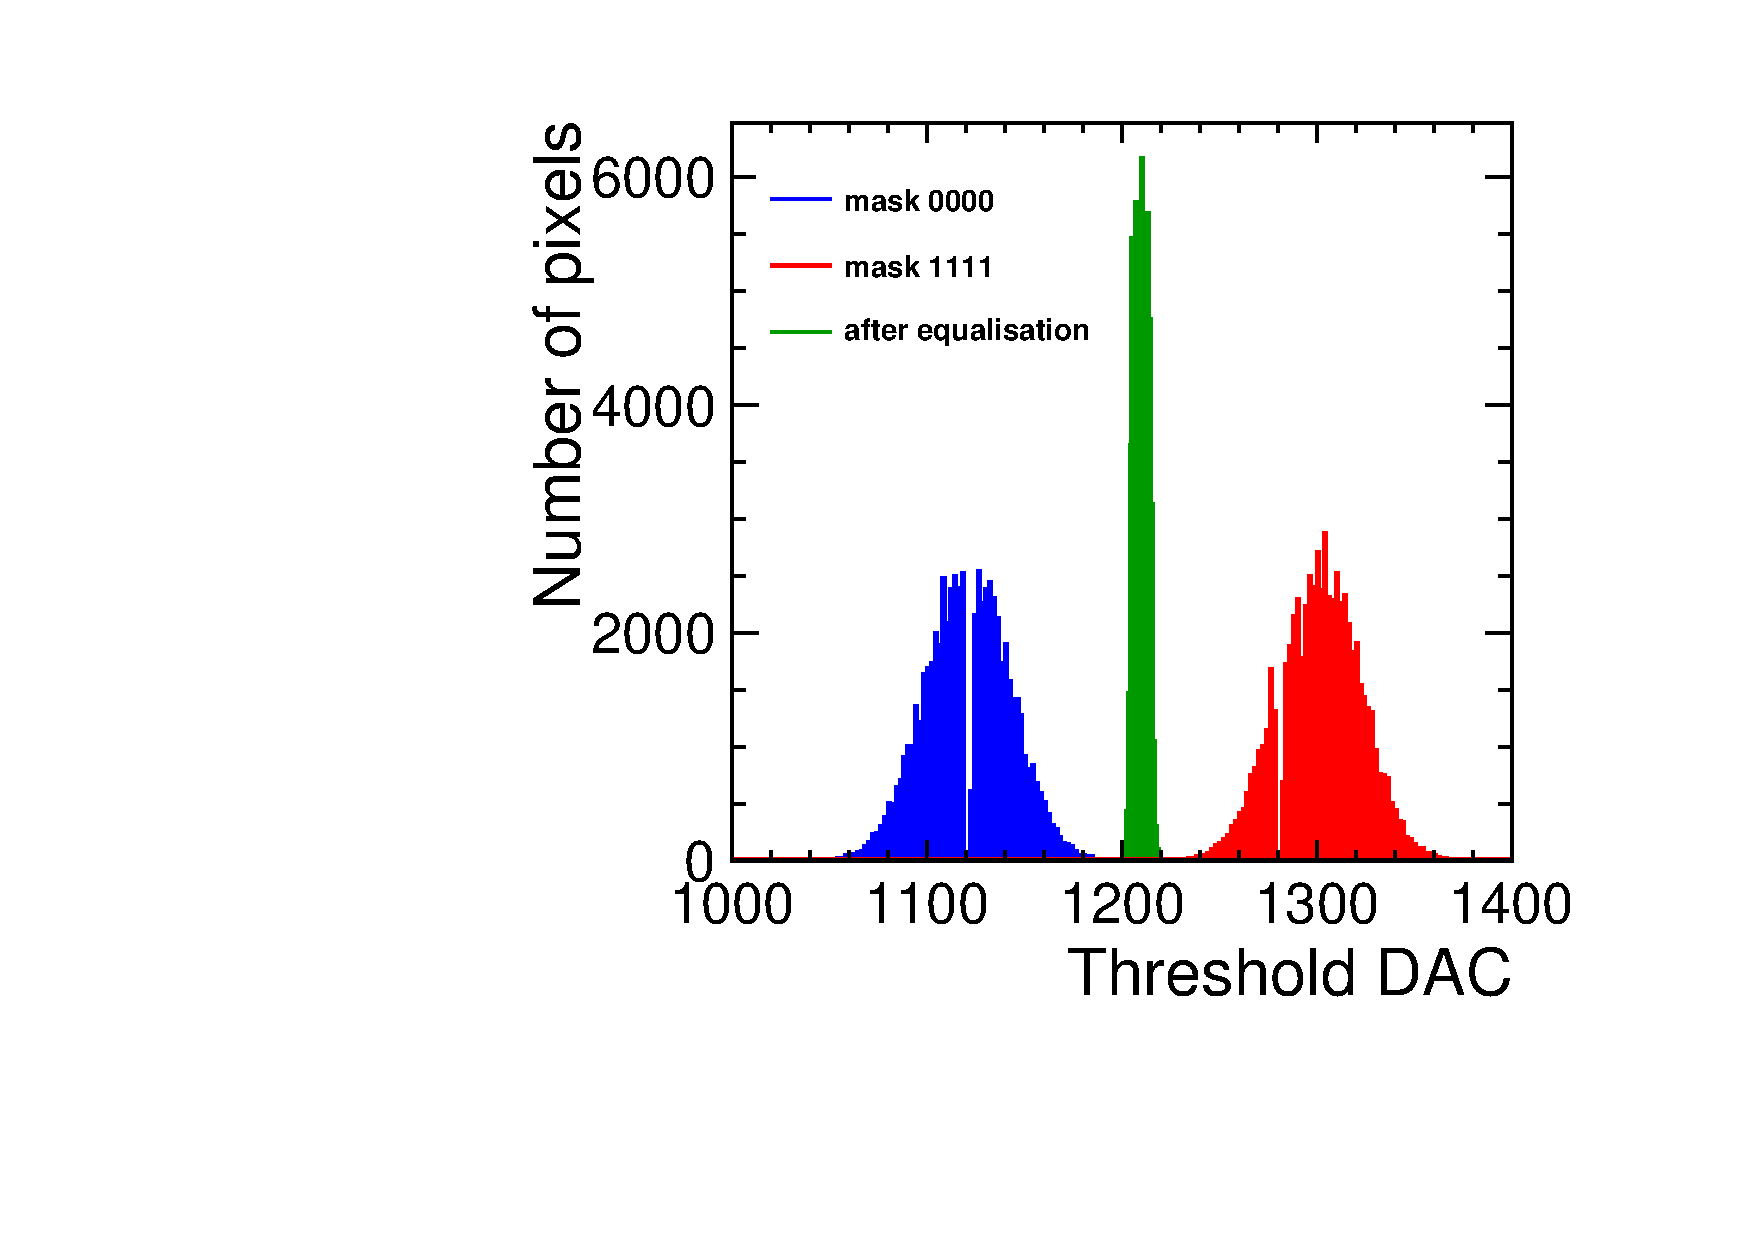
\includegraphics[width=0.6\textwidth]{./figures/Calibration/THLequalisation_W2_J5.pdf}
  \caption{Threshold equalisation for the assembly W2\_J5.}
  \label{fig:THLequalisation}
\end{figure}

\subsection{Calibration} \label{sec:calibration} The aim of the
calibration is to parametrise the measurements done by the readout
chip, namely the relationship between the threshold DAC and the TOT
with the energy deposited in the sensor (in \kev or number of
collected charge) as well as the relation between the TOA measurement
and the time of arrival of the particle (in seconds).

The calibration can be achieved using two main methods. The first one
consists of the use of photons from radioactive sources with a
characteristic decay energy or photons from X-ray fluorescence with a
characteristic emission energy~\cite{AlipourTehrani:2054922}. The
photon being stopped in the sensor, it deposits its full energy. Since
the energy of the photon is known, its relation to the TOT can be
characterised. The counting mode is used to calibrate the threshold.

The second method consists of the use of an internal analog test pulse
generator. The Timepix readout ASICs provide an internal test pulse
generator which can be used for calibration as well as equalisation of
the readout chip. In each pixel, a capacitor allows for injecting a
charge by switching a voltage over it. The charge injected is given by

\begin{equation}
  Q = C \cdot \Delta V \; ,
  \label{eq:testpulseCharge}
\end{equation}

where Q is the injected charge, C the injection capacitance and
$\Delta V$ the voltage applied. A priori, the injection capacitance is
unknown and its value varies from pixel to pixel but its value can be
measured.

\subsubsection{Energy calibration} \label{sec:EnergyCalibration}

For the energy calibration, the Timepix readout ASIC is operated in
the TOT mode. Data points obtained either by radioactive sources or
test-pulse injection are used to parametrise the relationship between
the energy deposited and the TOT measurement. Due to the non-linearity
of the Timepix charge pre-amplifier, this relationship is modeled as a
hyperbola. The function used to fit the data points is called a
\textit{surrogate function} and is defined as:

\begin{equation}
  \text{TOT} = a \, E + b - \frac{c}{E - t} \; ,
  \label{eq:TOTsurrogateFunction}
\end{equation}

where TOT denotes Time-Over-Threshold, $E$ the energy and $a, b, c, t$
are the parameters to be found~\cite{Jakubek2008155}. The inverse of
the surrogate function is defined as:

\begin{equation}
  E = { {t \cdot a - \text{TOT} -b + \sqrt{\left(b+t \cdot a -\text{TOT}\right)^2+4\cdot a \cdot c}} \over {2a} } \; ,
  \label{eq:inverseTOTsurrogateFunction}
\end{equation}

In \cref{eq:TOTsurrogateFunction}, for higher values of the energy,
the relationship between TOT and $E$ is linear with gradient $a$ and
intercept $b$ since the term $aE+b$ dominates. At low energy, the term
$c/(E-t)$ becomes important. The parameter $c$ defines the amount of
curvature in the function. An asymptote occurs at $E=t$. The point at
which the fit crosses the x-axis (TOT=0) corresponds to the threshold:
below the threshold no charge can be detected. The range for the TOT
and the boundary between low energy (non-linear response) and high
energy (linear response) depend on the clock frequency, the threshold
and the I\textsubscript{krum} values.

For the Timepix3 ASICs, the test-pulse injection is used for the
calibration of the assemblies. Test pulses with heights ranging from
$0\,\mv$ to $800\,\mv$ (corresponding to 0 electrons to 14000
electrons) are sent to each pixel. For each pulse height, 100
test-pulses are sent. The sum of the TOTs and also the sum of the
squared of the TOTs for each pulse height is recorded. The mean of the
TOT response and the standard deviations are then calculated. Finally,
the data are fitted with the surrogate function as given in
\cref{eq:TOTsurrogateFunction} for each pixel and the pixel-by-pixel
energy calibration of the assembly is determined.

\cref{tab:timepix3Operation} summarises the DAC settings used for the
operation of the Timepix3 assemblies in test beams. The same settings
are as well used for the calibration. \cref{fig:TOTcalib_55GNDGR100}
shows the pixel-by-pixel calibration for assembly 55-GNDGR-100
operated at two different threshold DACs of 1160 and 1190. For a
higher threshold, the curve is shifted towards higher energy values on
the x-axis but the slope (parameter $a$) remains the same.

\begin{table}[htbp]
  \centering
  \caption{DAC settings for the operation and calibration of the
    Timepix3 assemblies. VFBK is a programmable DAC to determine the
    baseline voltage of the chip.}
  \label{tab:timepix3Operation}
  \begin{tabular}{ c c c c }
    \toprule
    I\textsubscript{krum} & TOT/TOA Clock & FTOA Clock & VFBK \\
    \midrule
    10 & $40\,\megahertz$ & $640\,\megahertz$ & 150 \\
    \bottomrule
  \end{tabular}
\end{table}

\begin{figure}[htbp] \centering
  \begin{subfigure}[b]{0.45\textwidth}
    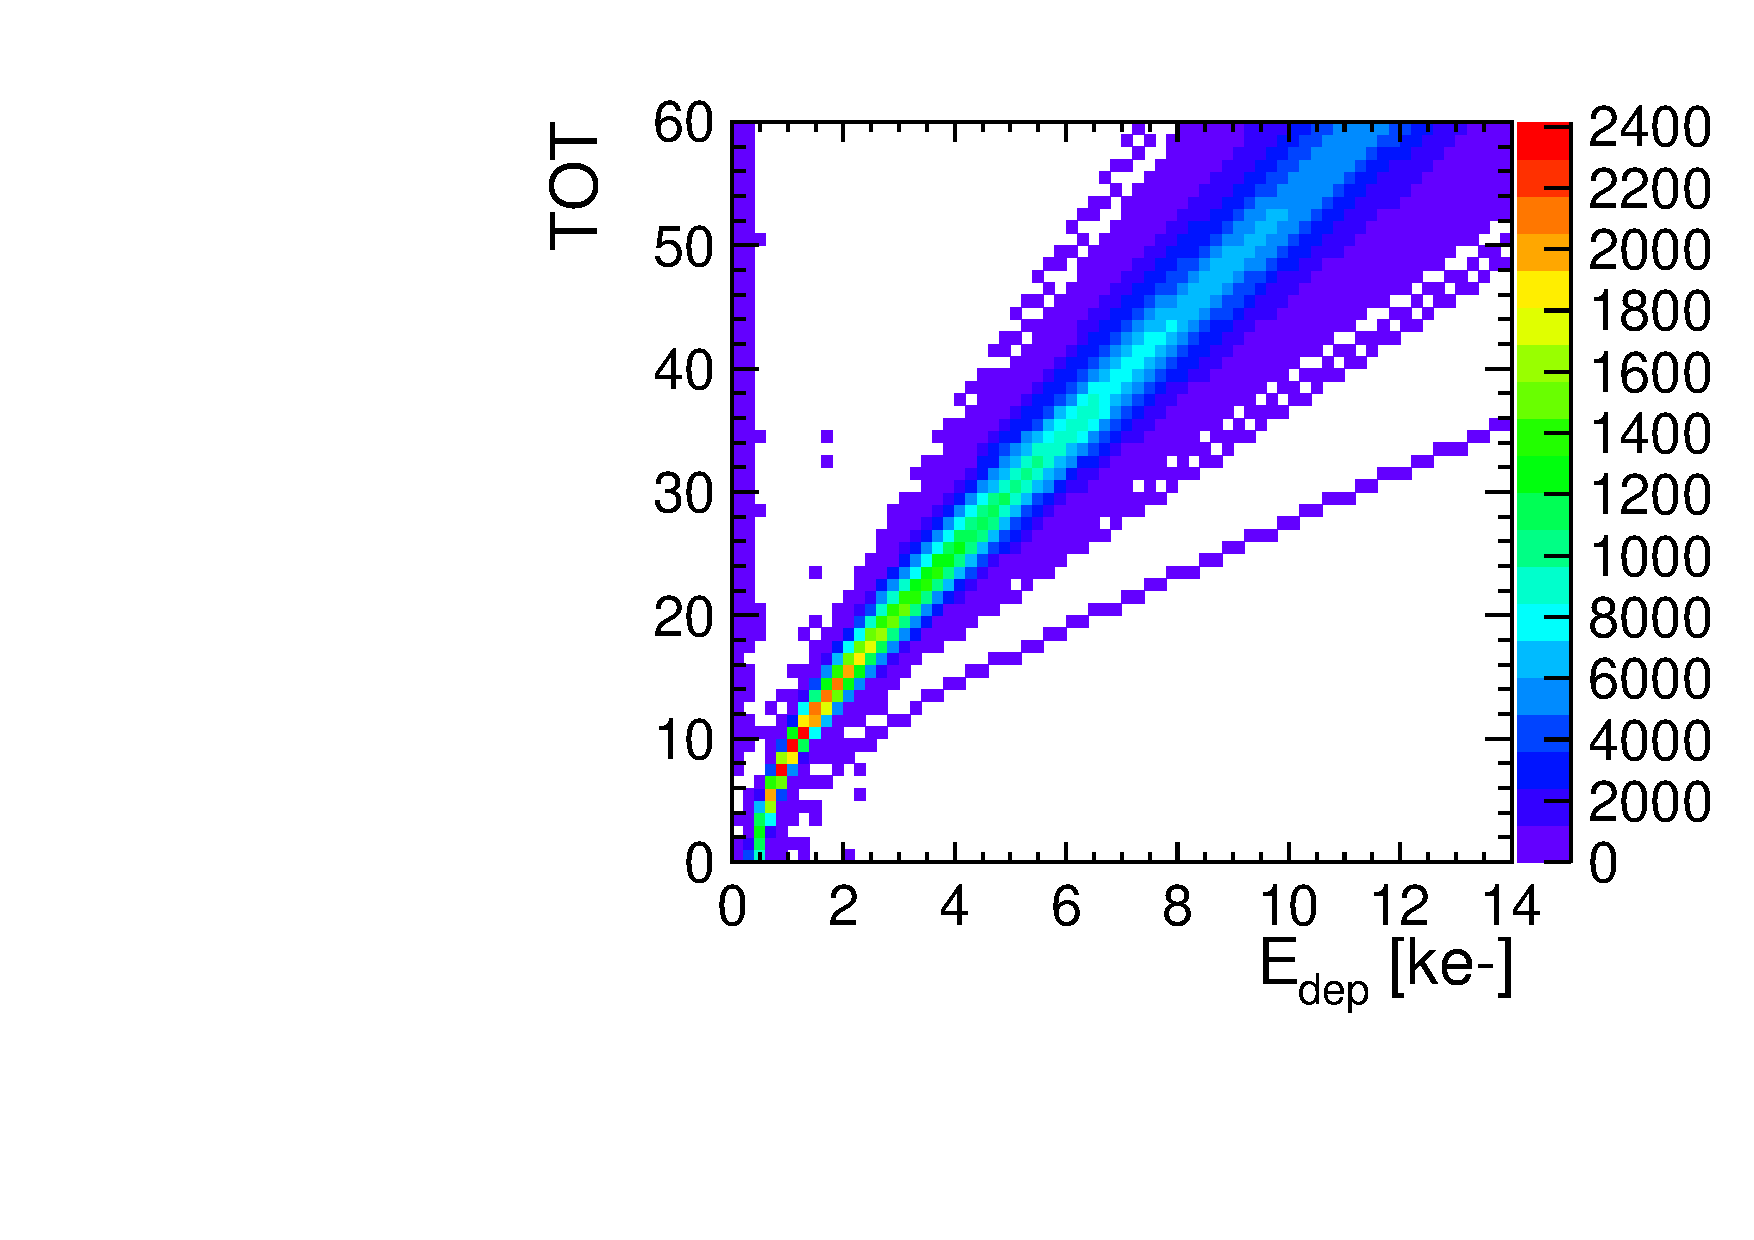
\includegraphics[width=\textwidth]{./figures/Calibration/TOTcalibration_W0005_E02_thresh1160.pdf}
    \caption{}
  \end{subfigure} \hfill
  \begin{subfigure}[b]{0.45\textwidth}
    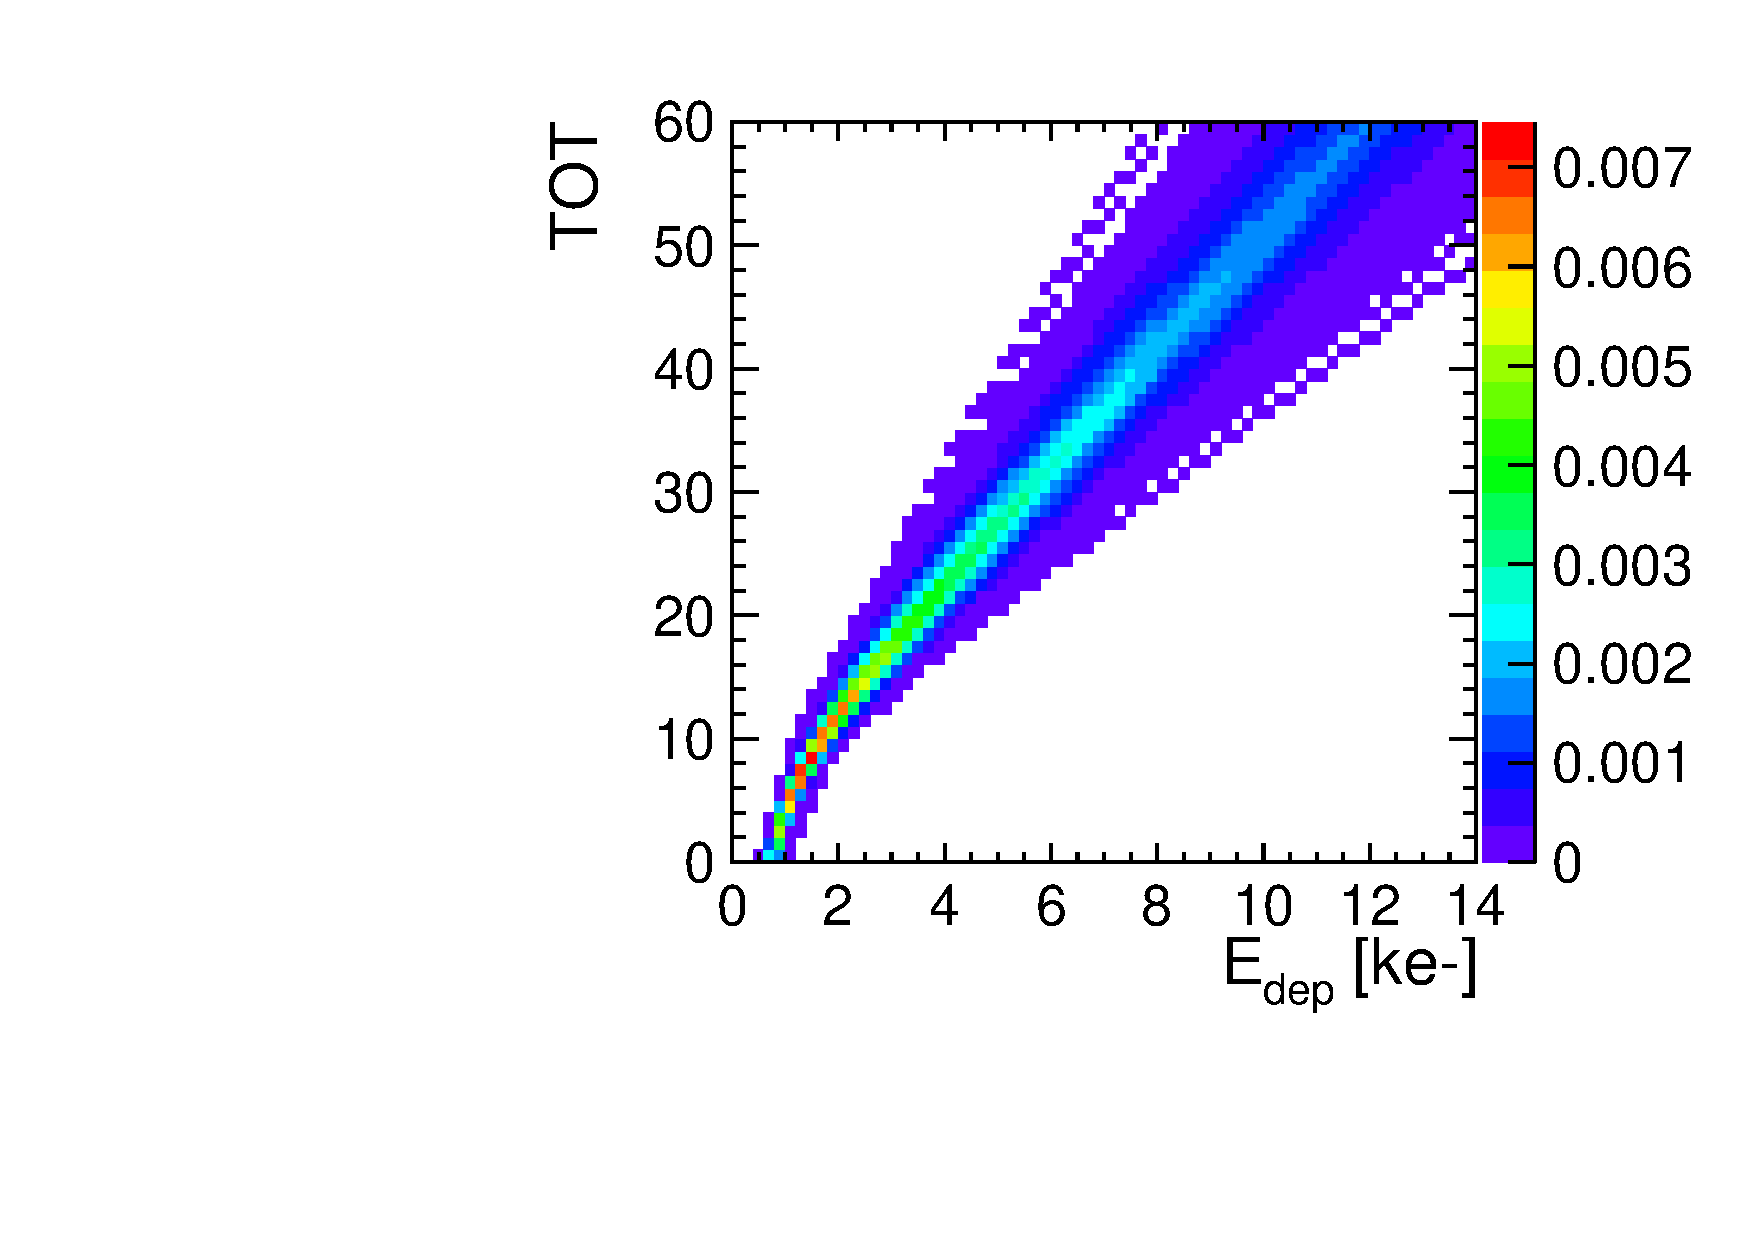
\includegraphics[width=\textwidth]{./figures/Calibration/TOTcalibration_W0005_E02_thresh1190.pdf}
    \caption{}
  \end{subfigure}
  \caption{Pixel-by-pixel calibration of the TOT for assembly
    55-GNDGR-100 operated at the threshold DACs of (a) THL=1160 and
    (b) THL=1190.}
  \label{fig:TOTcalib_55GNDGR100}
\end{figure}

The calibration for the other assemblies are given in \cref{sec:appendixFE_electronics}.


\subsubsection{Threshold calibration} \label{sec:threshold}


The operating threshold DAC (Digital-to-Analog Converter) set in each
Timepix/Timepix3 readout chip can be translated into an effective
energy and used as a data point for the surrogate fit at the
crossing-point on the $x$-axis. The counting (Medipix) mode is used
for this measurement.  

For the Timepix assemblies, the calibration is done with radioactive
sources since the test-pulse calibration is not possible due to the
choice of the I\textsubscript{krum} value. The assembly is exposed to
photons of a characteristic energy and the threshold DAC is scanned
from a level of no counts (threshold above the signal) to a level
where all the pixels count (threshold close to the noise level)
resulting in an S-shaped curve as shown in
\cref{fig:scurve_example}. At the maximum gradient of the S-curve, the
threshold DAC corresponds to the photon energy. The derivative of the
S-curve is a Gaussian as shown in \cref{fig:deriv_example} with a mean
at the maximum gradient of the S-curve. The derivative at each point
of the S-curve corresponds to the slope of the line connecting it to
its neighbour.

\begin{figure}[htbp] \centering
  \begin{subfigure}[b]{0.45\textwidth}
    \begin{tikzpicture} \node[anchor=south west,inner sep=0] (image)
      at
      (0,0){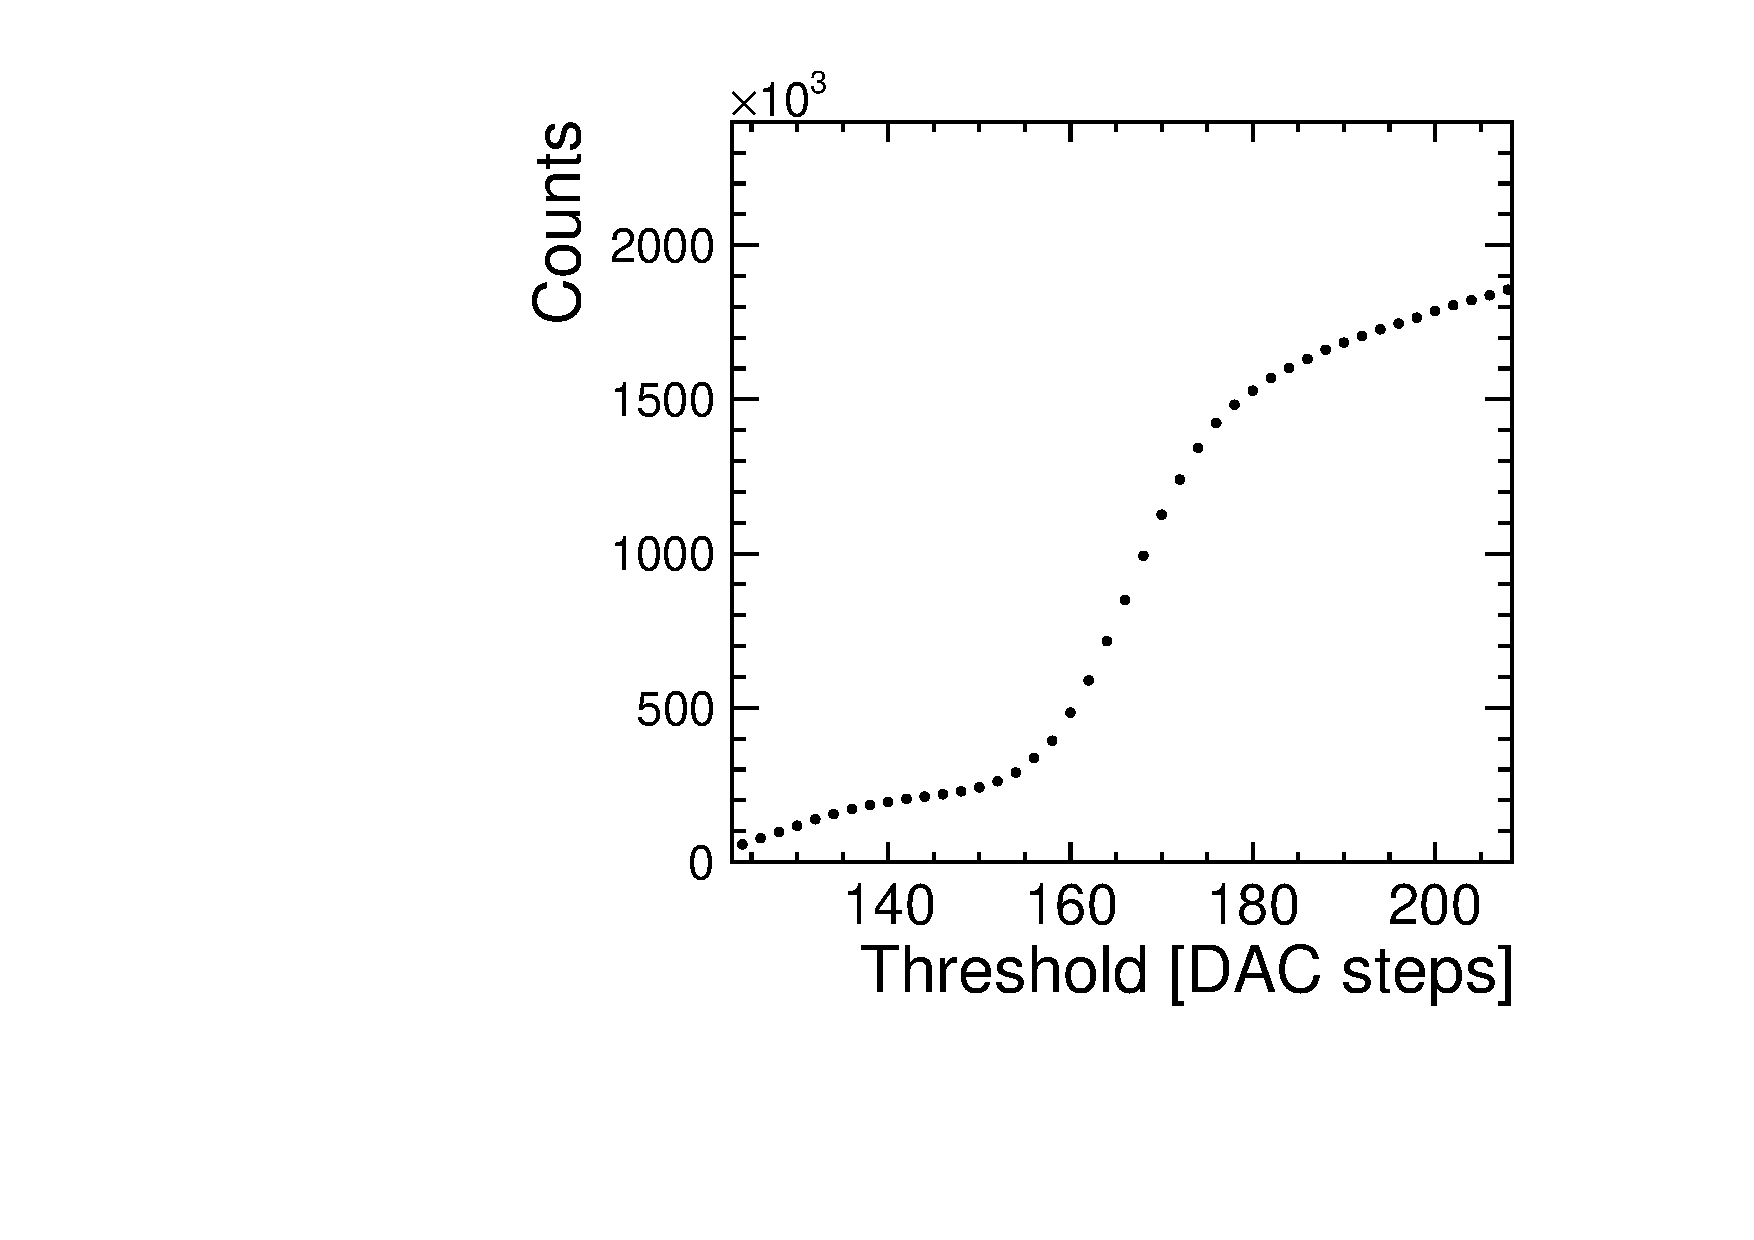
\includegraphics[width=\textwidth]{./figures/Calibration/L04-W0125_scurve_In.pdf}};
      % \draw[->,line width=.4pt, color=black](1.8, 1.4) -- (2.4, 1.4);
      \node[left, color=black] at (1.9, 1.6) {$K_{\beta}$}; %\draw[->,line
      width=.4pt, color=black](3, 2.7) -- (3.7, 2.7); \node[left,
      color=black] at (3.5, 2.7) {$K_{\alpha}$};
    \end{tikzpicture}
    \caption{Measured S-curve}
    \label{fig:scurve_example}
  \end{subfigure} \hfill
  \begin{subfigure}[b]{0.45\textwidth}
    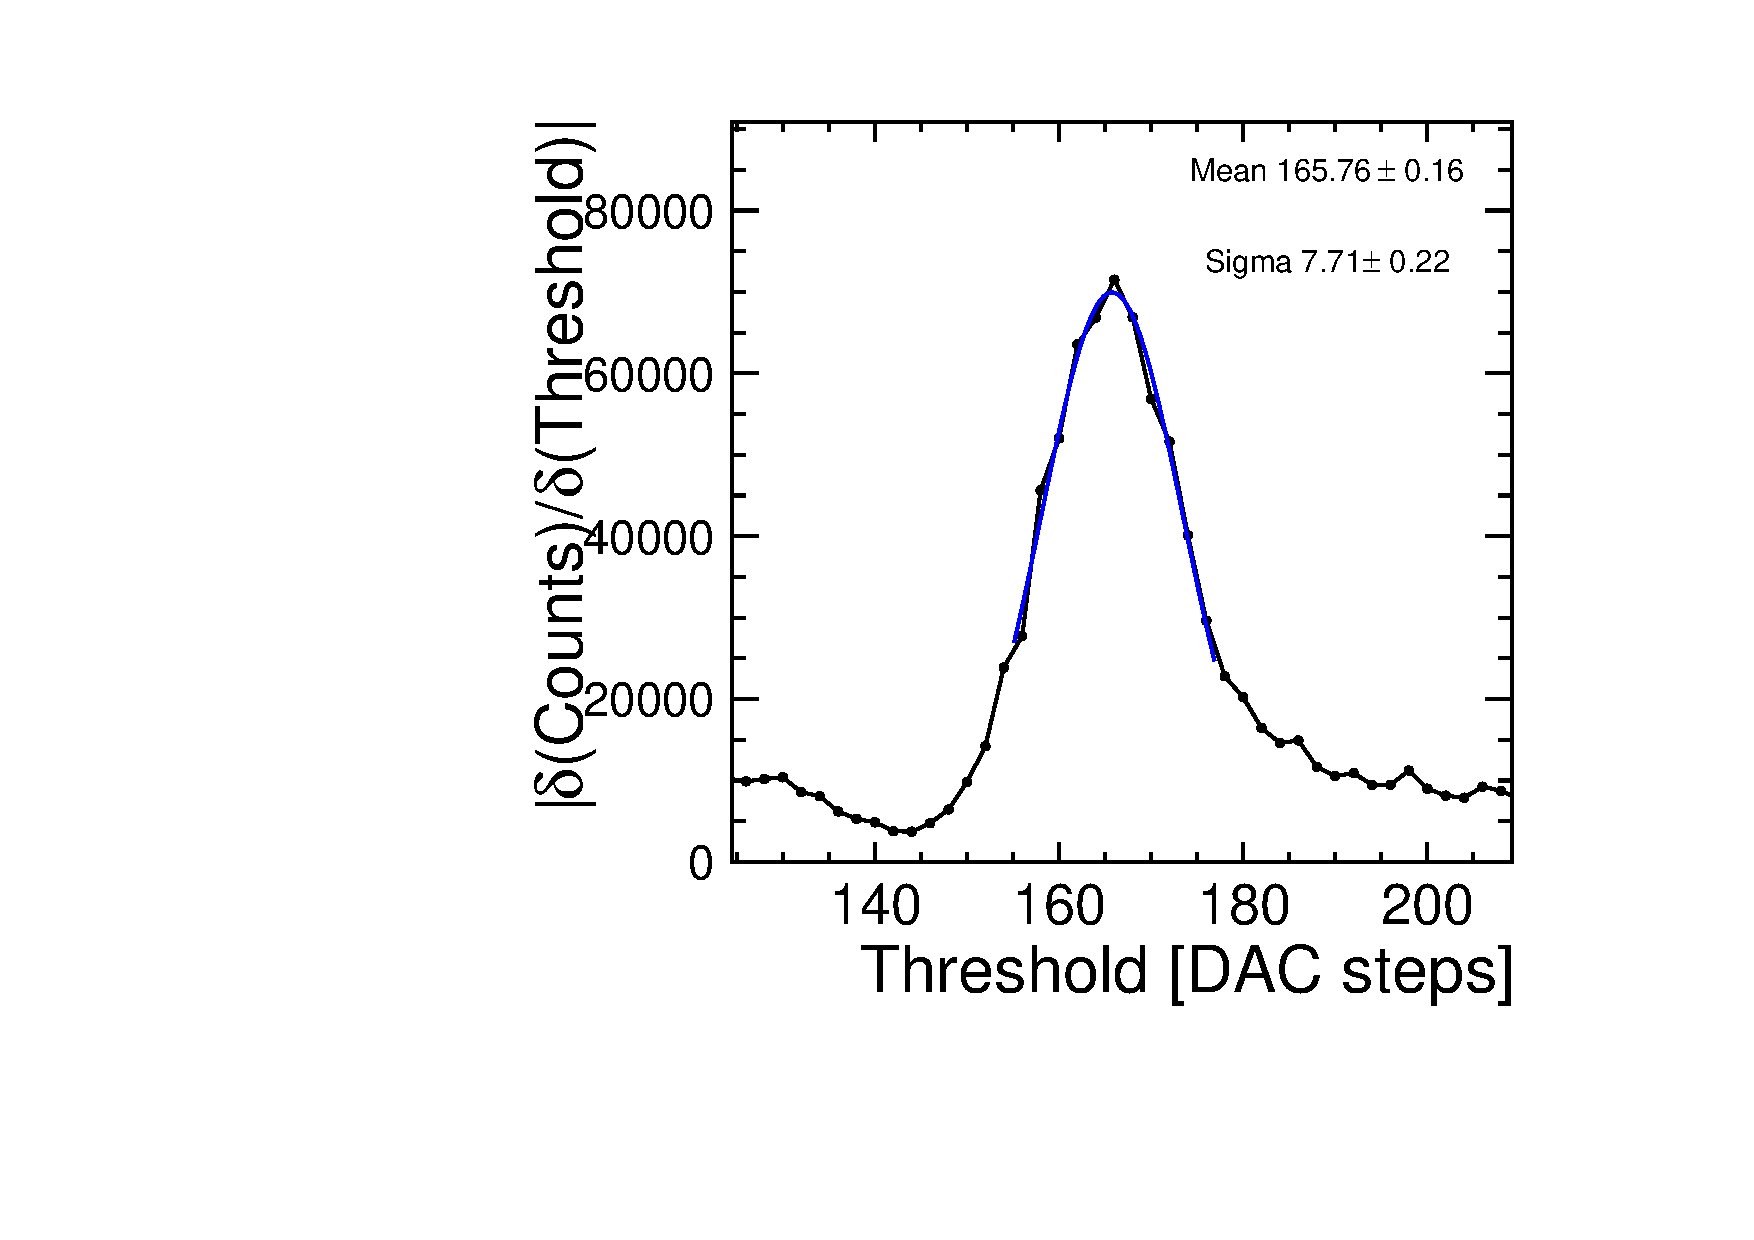
\includegraphics[width=\textwidth]{./figures/Calibration/L04-W0125_scurveDeriv_In.pdf}
    \caption{Derivative of the S-curve}
    \label{fig:deriv_example}
  \end{subfigure}
  \caption{An example of a measured S-curve (a) and its derivative
    fitted with a Gaussian function (b) for a Timepix readout ASIC
    (L04-W0125) using the Indium target. $K_{\alpha}$ corresponds to
    the strongest X-ray spectral line for the bombarded target. The
    smaller peak for $K_{\beta}$ is ignored. For Timepix
    assemblies. The Pixelman software~\cite{1748-0221-6-01-C01046}
    provides the \emph{DACs Scan} plug-in which was used to scan the
    threshold DAC value and save the hit maps in a text file. The
    threshold calibration was done at CERN using the XRF targets. This
    measurement was performed globally for each assembly. The
    threshold DAC is scanned with a step size of 2.}
  \label{fig:scurve_deriv_example}
\end{figure}

A linear fit is used to parametrise the relationship between the
photon energy and the threshold DAC given by the mean of the
derivative of the S-curves:
\begin{equation}
  THL_{DAC}=p \; THL_{\kev} + q \; ,
  \label{eq:THLDAC}
\end{equation}
where $THL_{DAC}$ is the threshold DAC and $THL_{\kev}$ its conversion
into an energy. \cref{fig:THLcalib_A06} shows an example of the
threshold calibration obtained for a Timepix chip (assembly
A06-W0110). Each point used for the fit corresponds to the mean of the
Gaussian fitted to the derivative of the S-curve for each target. The
error on each point corresponds to the error on the mean of the fitted
Gaussian.

\begin{figure}[htbp]
  \centering
  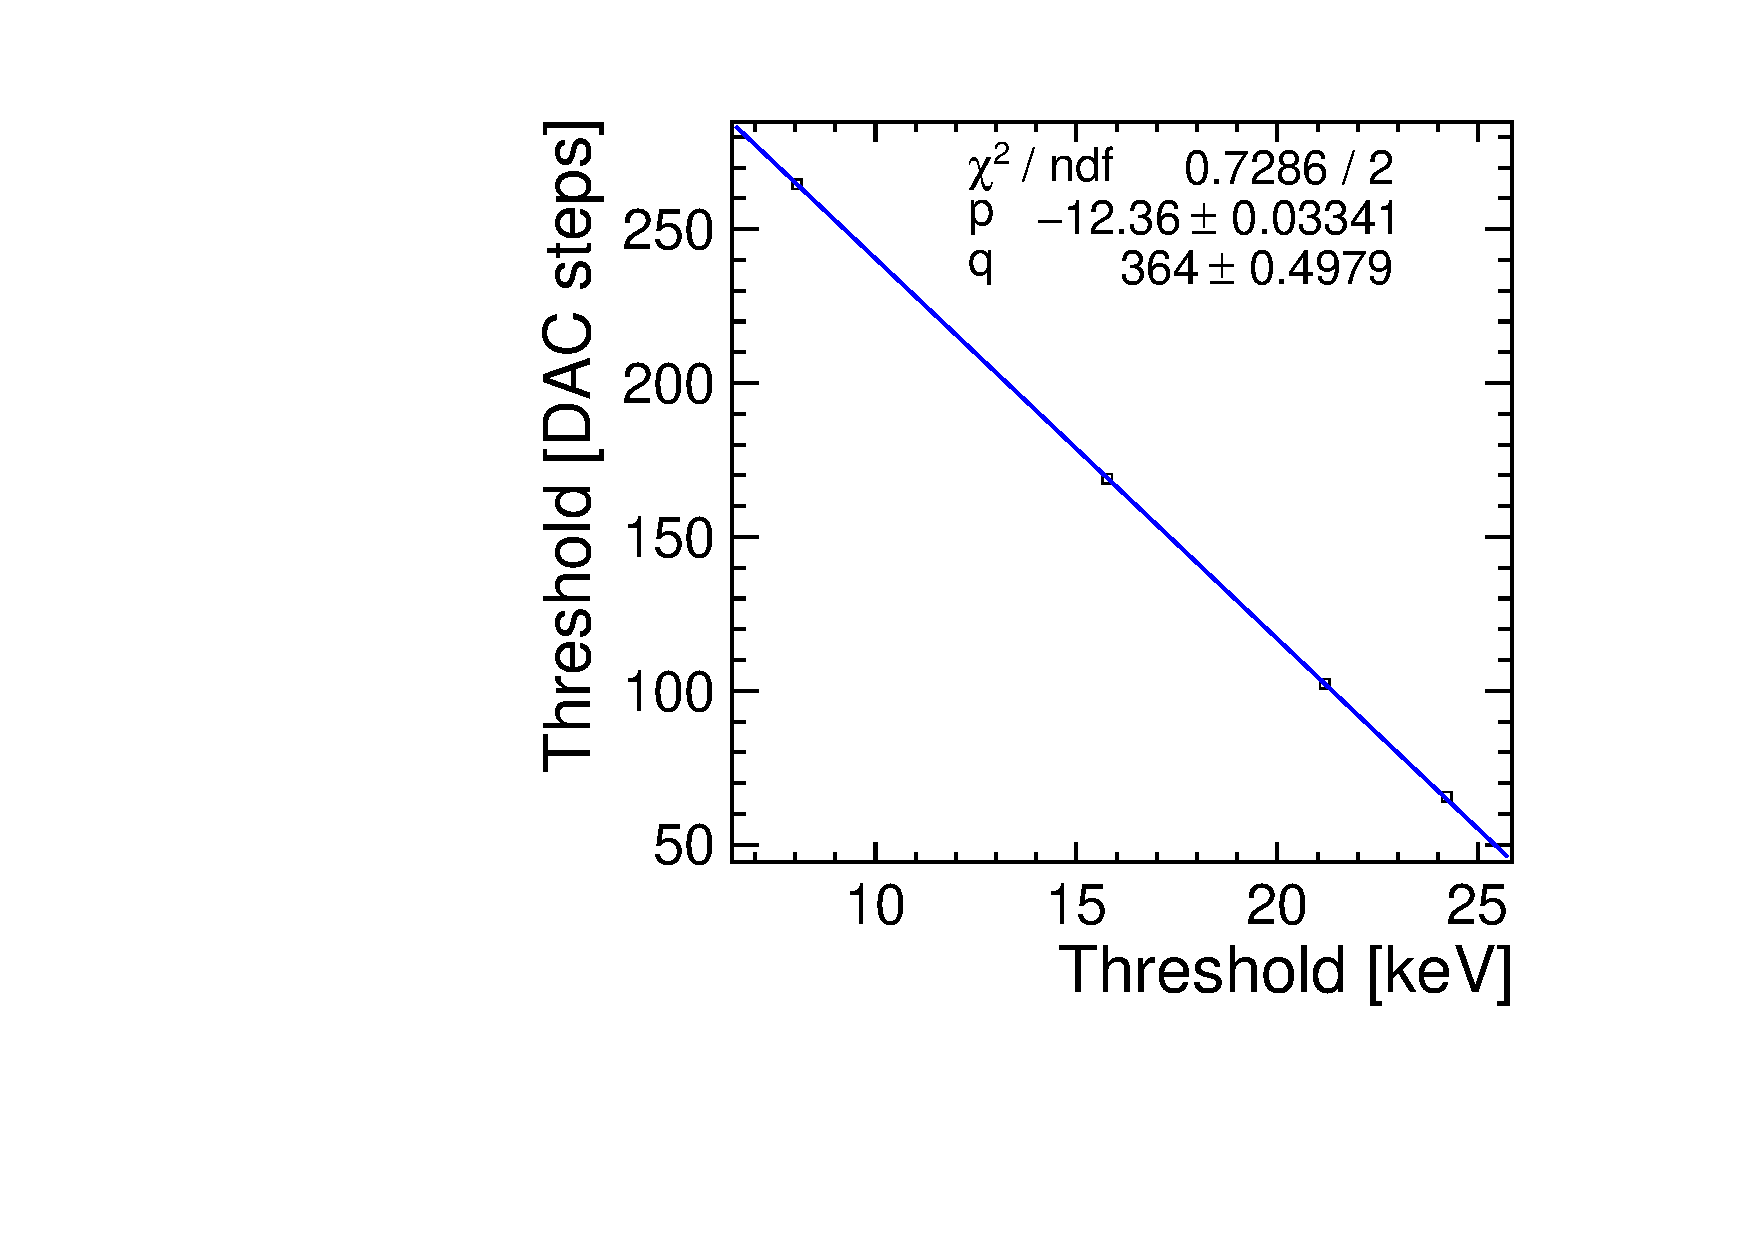
\includegraphics[width=0.5\textwidth]{./figures/Calibration/A06-W0110_THLcalibration.pdf}
  \caption{Threshold calibration for A06-W0110. Each point corresponds
    to the maximum gradient of the S-curve for each target (Cu, Zr, Pd
    and In). A linear function as described in \cref{eq:THLDAC} was
    used to fit the data points and obtain the parameters $p$ and
    $q$.}
  \label{fig:THLcalib_A06}
\end{figure}

The operating threshold DAC for each assembly was converted to an
energy by solving \cref{eq:THLDAC} for $THL_{\kev}$ with
$THL_{DAC}=THL_{DAC}^{op}$. The error on the evaluated threshold in energy
($THL_{\kev}^{op}$) is obtained by the propagation of errors for the
inverse of \ref{eq:THLDAC}:
\begin{equation}
  \sigma_{THL_{\kev}}^2(THL_{DAC})={{{(THL_{DAC}-q)^2} \over {p^4}} \sigma_{p}^2} +
        {\frac{1}{p^2} \sigma_{q}^2}+
        {2 {{THL_{DAC}-q} \over p^3} \sigma_{pq}^2} \; ,
        \label{eq:THLerror}
\end{equation}
where $p$, $q$ are given by the linear fit using \cref{eq:THLDAC} with
standard deviations $\sigma_{p}$, $\sigma_{q}$ and covariance
$\sigma_{pq}$.

% \begin{table}[htbp]
%   \caption{Threshold fit parameters $p$ and $q$, the operating
%     threshold DAC and its conversion into energy.}
%   \label{tab:evalTHL} 
%   \centering
%   \begin{tabular}{ c c c c c }
%     \toprule
%     Assembly & $p$ [DAC steps/\kev] & $q$ [DAC steps] & $THL_{DAC}^{op}$ [DAC steps] & $THL_{\kev}^{op}$ [\kev] \\
%     \midrule
%     A06-W0110 & $-12.36\pm0.03$ & $364.0\pm0.50$ & 326 & $3.077\pm0.033$ \\
%     C04-W0110 & $-11.8\pm0.02$ & $441.6\pm0.42$ & 405 & $3.102\pm0.030$ \\
%     L04-W0125 & $-11.68\pm0.02$ & $448.6\pm0.31$ & 410 & $3.303\pm0.023$ \\
%     B06-W0125 & $11.58\pm0.037$ & $390.6\pm0.80$ & 435 & $3.836\pm0.057$ \\
%     \bottomrule
%   \end{tabular}
% \end{table}

For further verification of these results, the Timepix DAC step gain
for each assembly is calculated to be around
24~$\pm$e\textsuperscript{-}/step, in agreement
with~\cite{art:tmpx}. The width of the derivative of the S-curves
shows the error at the front-end of the assembly. For all assemblies
it varies between 7 to 11 DAC values which corresponds to 170 to 270
electrons, again in agreement with~\cite{art:tmpx} (the error is
obtained by error propagation of \cref{eq:THLDAC}).


For Timepix3 assemblies, the threshold is calibrated using test pulses
at four different heights corresponding to 0, 1000, 3000 and 6000
electrons. For each pulse height, 200 pulses are sent to the pixels in
the diagonal of the matrix. The threshold is scanned, like for Timepix
assemblies, from a level of no counts to a level where all the pixels
count. The S-curves and their derivatives are calculated. Finally, a
linear fit is used to parametrise the relationship between the pulse
height and the threshold DAC.

The threshold calibration for 55-GNDGR-100 is shown in
\cref{fig:THLcalib_55-GNDGR-100} (for the other assemblies refer to
\cref{fig:Timepix3_THL_Calibration}). For the Timepix3 ASIC has a DAC
step gain of around $11\pm$e-/step is calculated. The noise measured
at the front-end corresponds to 80 to 90
electrons. \cref{tab:NominalThreshold} summarises the conversion of
the threshold DAC into energy for the different assemblies at nominal
conditions.

\begin{figure}[htbp]
  \centering
  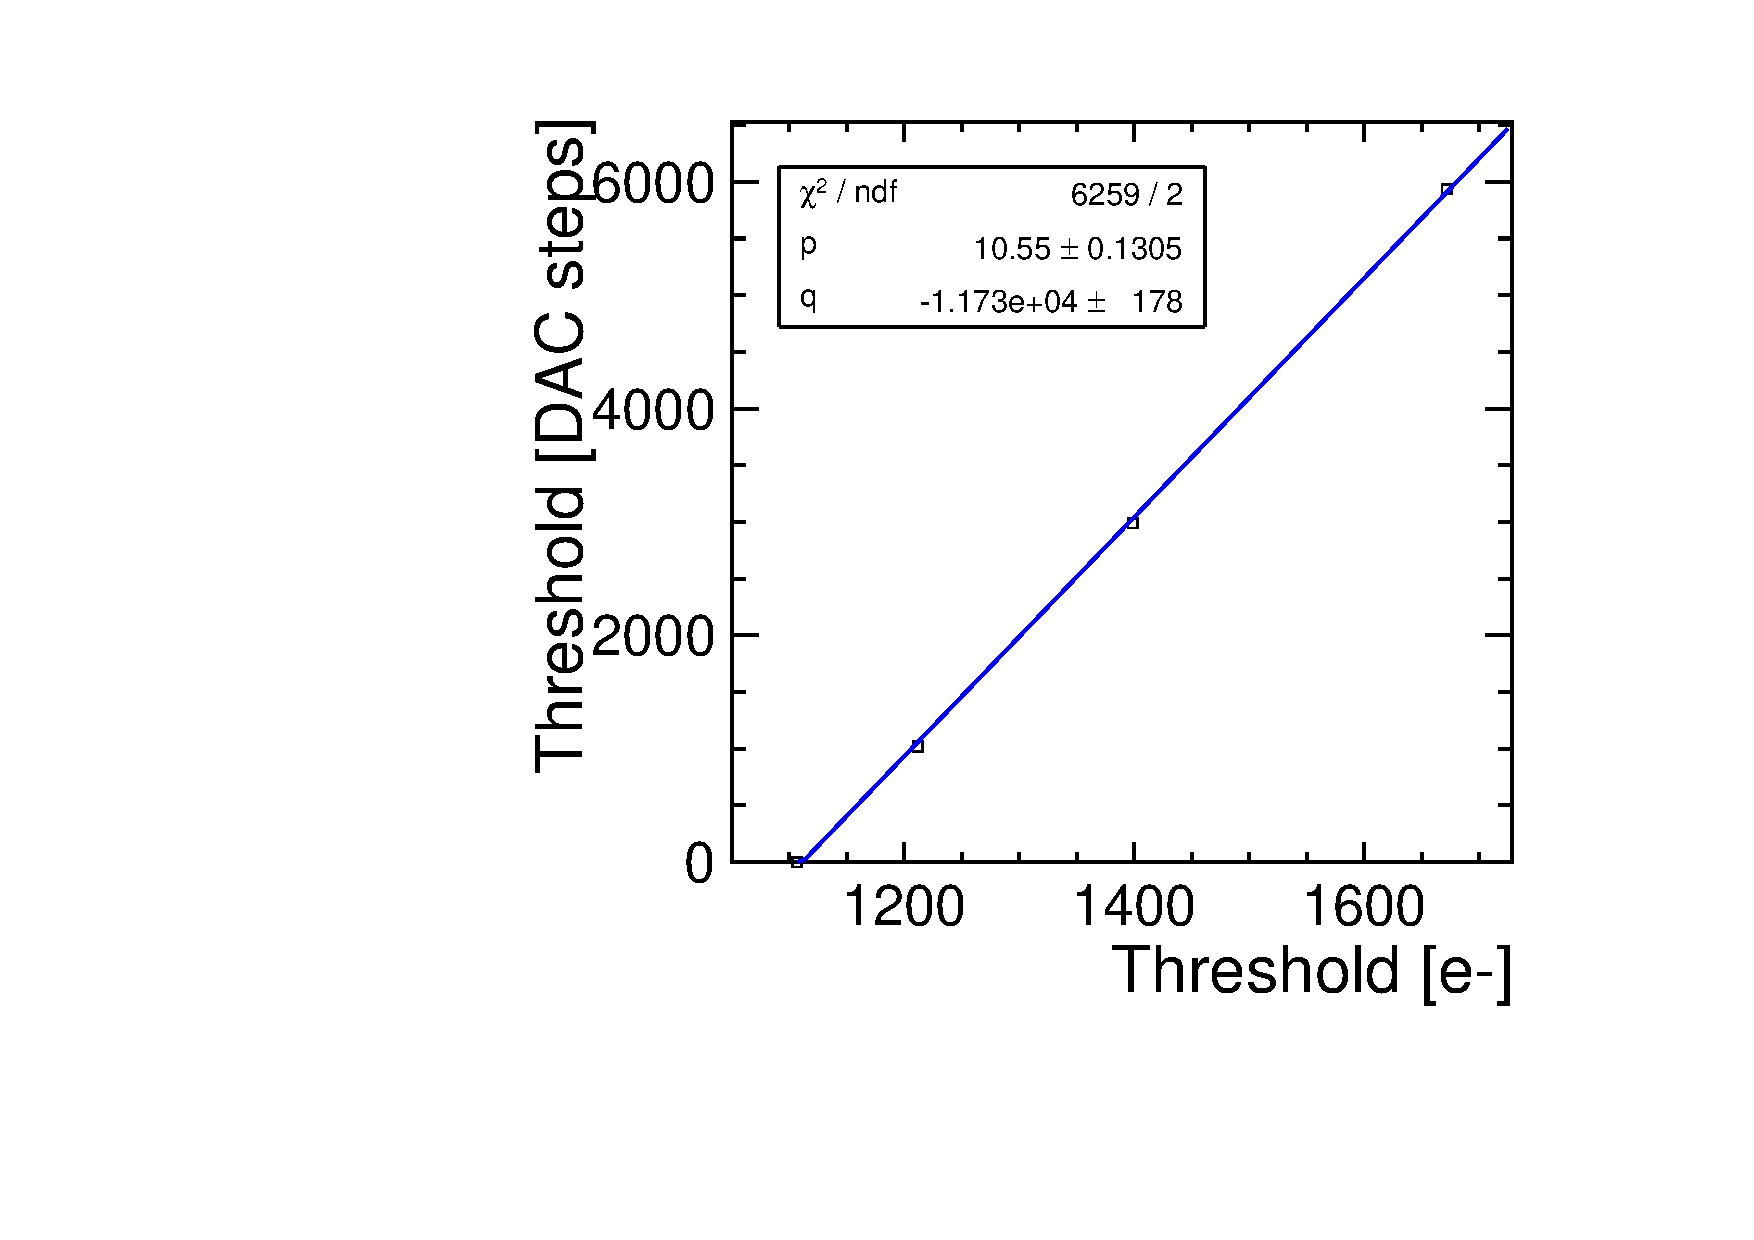
\includegraphics[width=0.5\textwidth]{./figures/Calibration/THLcalibration_W0005_E02.pdf}
  \caption{Threshold calibration for 55-GNDGR-100. Each point
    corresponds to the maximum gradient of the S-curve for each pulse
    height. A linear function as described in \cref{eq:THLDAC} was
    used to fit the data points and obtain the parameters $p$ and $q$.}
  \label{fig:THLcalib_55-GNDGR-100}
\end{figure}

\begin{table}[htbp]
  \centering
  \caption{Advacam active-edge n-in-p planar pixel sensor assemblies. The edge distance is defined by the distance between the last pixel implant and the physical sensor edge.}
  \label{tab:NominalThreshold}
  \resizebox{\textwidth}{!}{\begin{tabular}{lccc}
      \toprule
      Assembly & Nominal THL\textsubscript{DAC}\textsuperscript{op} [DAC steps] & Nominal THL\textsubscript{e-}\textsuperscript{op} [electrons]\\
      \midrule
      20-NGR & 1190 & 466.5\\
      23-FGR & 1187 & 532.4\\ \hline
      28-GNDGR & 1133 & 517.8\\
      55-GNDGR & 1148 & 553.7\\
      55-GNDGR-100 & 1160 & 537.9\\ \hline
      55-GNDGR-150 & 1153 & 441.2\\
      \bottomrule
  \end{tabular}}
\end{table}



%%%%%%%%%%%%%%%%%%%%%%%%%%%%%%%%%%%%%%%%%%%%%%%%%%
\begin{table}[htbp]
  \centering
  \caption{}
  \label{tab:THLcalibration}
  \begin{tabular}{lcccc}
    \toprule
    Assembly & p [DAC steps/e\textsuperscript{-}] & q [DAC steps] & THL\textsubscript{DAC}\textsuperscript{op} [DAC steps] & THL\textsubscript{e-}\textsuperscript{op} [e\textsuperscript{-}] \\
    \midrule
    W19\_G7 & $0.087\pm0.000$ & $1144.037\pm0.005$ & 1190 & $526.230\pm0.649$ \\
    W19\_F7 & $0.092\pm0.000$ & $1131.874\pm0.009$ & 1187 & $600.406\pm0.551$ \\
    W19\_L8 & $0.090\pm0.000$ & $1082.057\pm0.005$ & 1133 & $568.506\pm0.538$ \\
    W19\_C7 & $0.091\pm0.000$ & $1092.887\pm0.005$ & 1148 & $608.700\pm0.488$ \\
    W5\_E2 &  $0.095\pm0.000$ & $1106.921\pm0.004$ & 1160 & $561.019\pm0.712$ \\
    W5\_F1 & $0.089\pm0.000$ & $1103.618\pm0.004$ & 1153 & $554.885\pm0.493$ \\
    W2\_J5 & $-0.109\pm0.000$& $1232.643\pm0.034$ & 1170 & $565.723\pm1.560$\\
    \bottomrule
  \end{tabular}
\end{table}

\begin{table}[htbp]
  \centering
  \caption{}
  \label{tab:THLcalibration_noise}
  \begin{tabular}{lcccc}
    \toprule
    Assembly & Baseline mean [DAC steps] & Threshold DAC step [e\textsuperscript{-}] & Noise [DAC steps] & Noise [e\textsuperscript{-}] \\
    \midrule
    W19\_G7 & $1143.992\pm0.005$ & $11.450\pm0.000$ & $6.864\pm0.005$ & $78.585\pm0.056$ \\
    W19\_F7 & $1131.664\pm0.009$ & $10.892\pm0.000$ & $7.060\pm0.009$ & $76.891\pm0.098$ \\
    W19\_L8 & $1081.998\pm0.005$ & $11.160\pm0.000$ & $6.996\pm0.005$ & $78.078\pm0.058$ \\
    W19\_C7 & $1092.825\pm0.005$ & $11.044\pm0.000$ & $7.413\pm0.005$ & $81.870\pm0.051$ \\
    W5\_E2  & $1106.895\pm0.004$ & $10.570\pm0.000$ & $7.155\pm0.004$ & $75.628\pm0.046$ \\
    W5\_F1  & $1103.591\pm0.004$ & $11.237\pm0.000$ & $6.711\pm0.004$ & $75.408\pm0.046$ \\
    W2\_J5  & $1231.70\pm0.034$ & $-9.177\pm0.000$ & $11.826\pm0.041$ & $108.53\pm0.379$ \\
    \bottomrule
  \end{tabular}
\end{table}


\section{Calibrated test beam data}

The test pulse calibration as described in
\cref{sec:EnergyCalibration} is applied to the data from test beams in
order to convert the energy deposited by the MIP
particles. \cref{sec:testBeamDataCalibrated_vs_G4} compares the
calibrated data with the \textsc{Geant4} energy deposition using the
PAI physics list (c.f. \cref{sec:Silicon_Geant4}) for $50\,\micron$,
$100\,\micron$ and $150\,\micron$ thick planar sensors. There is a
good agreement in terms of the most probable value (MPV) and the
full-width-at-half-maximum (FWHM) in both simulation and data.

\begin{figure}[htbp] \centering
  \begin{subfigure}[b]{0.33\textwidth}
    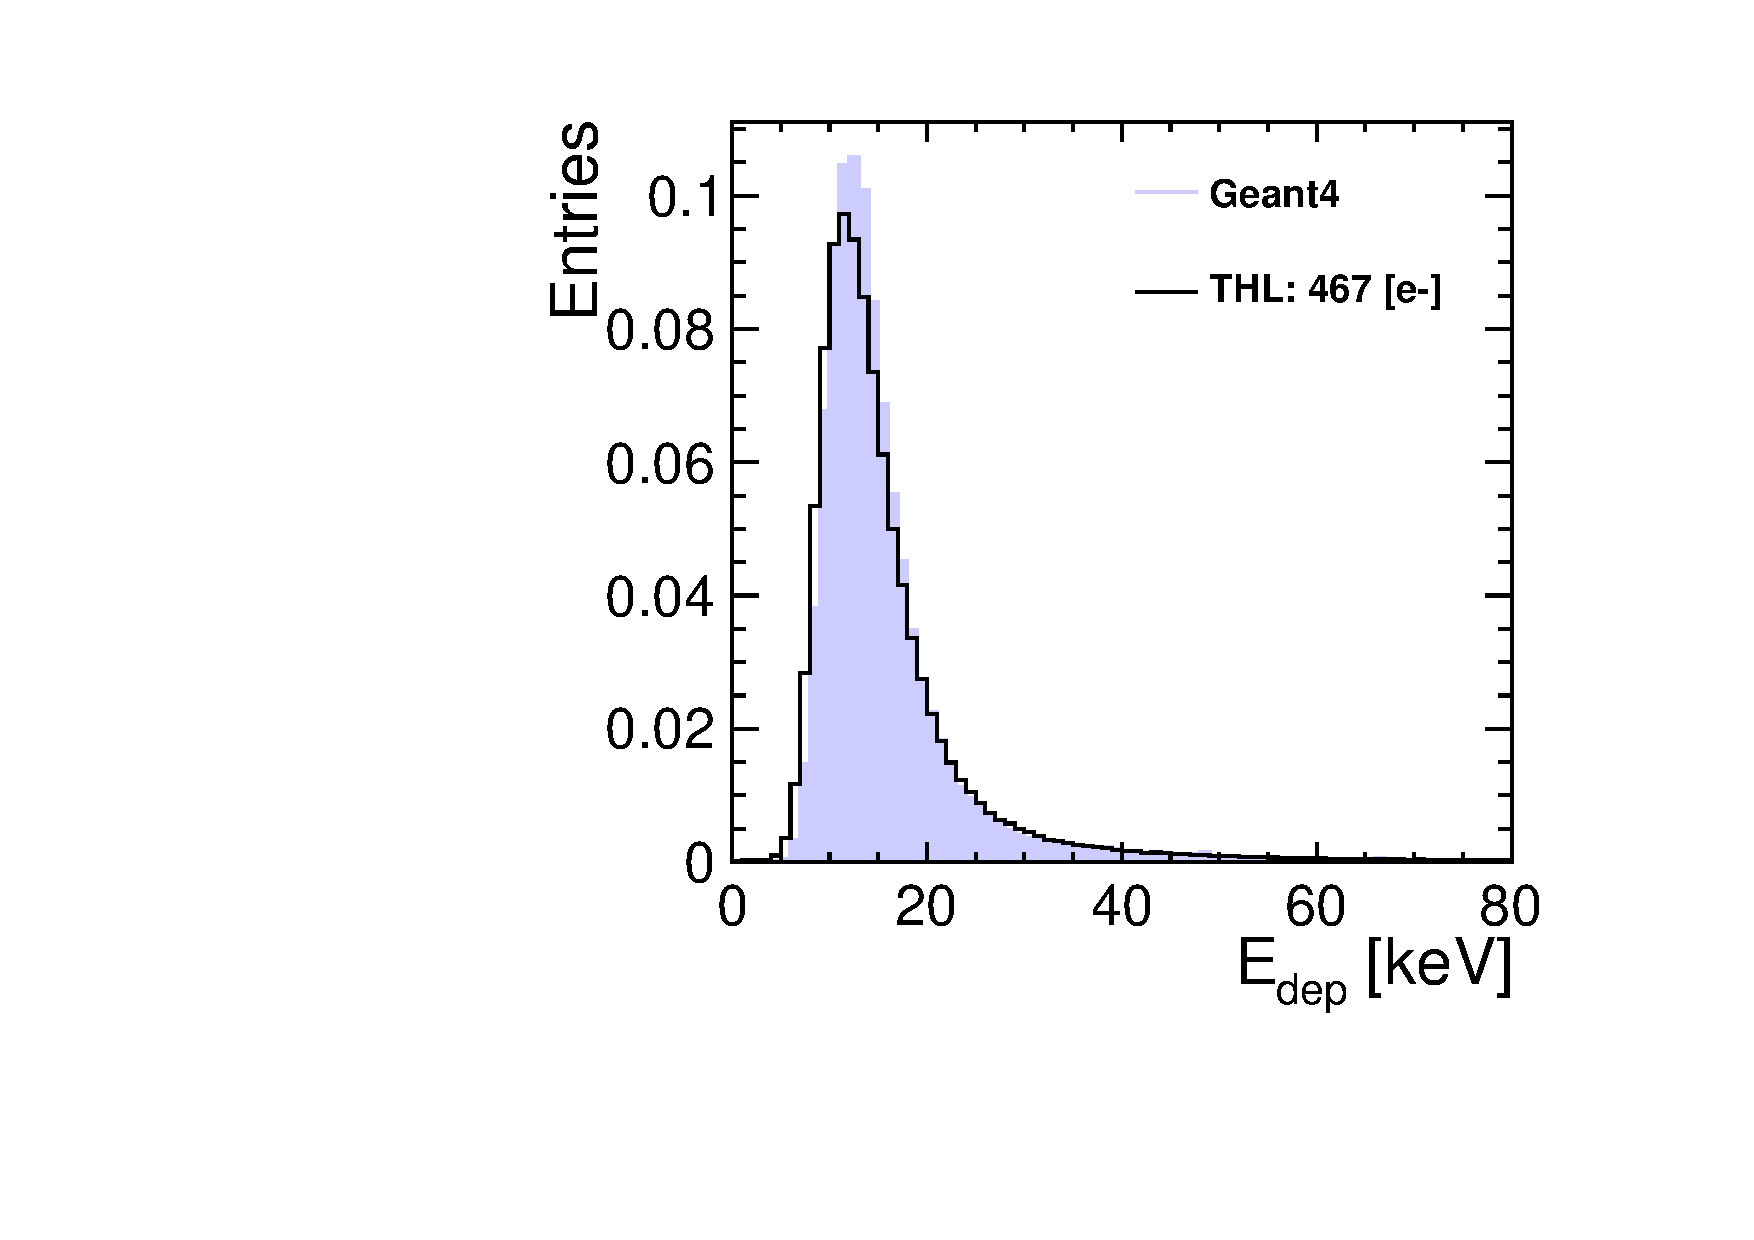
\includegraphics[width=\textwidth]{./figures/Calibration/Edep_G4_W0019_G07.pdf}
    \caption{55-GNDGR}
  \end{subfigure} \hfill
  \begin{subfigure}[b]{0.33\textwidth}
    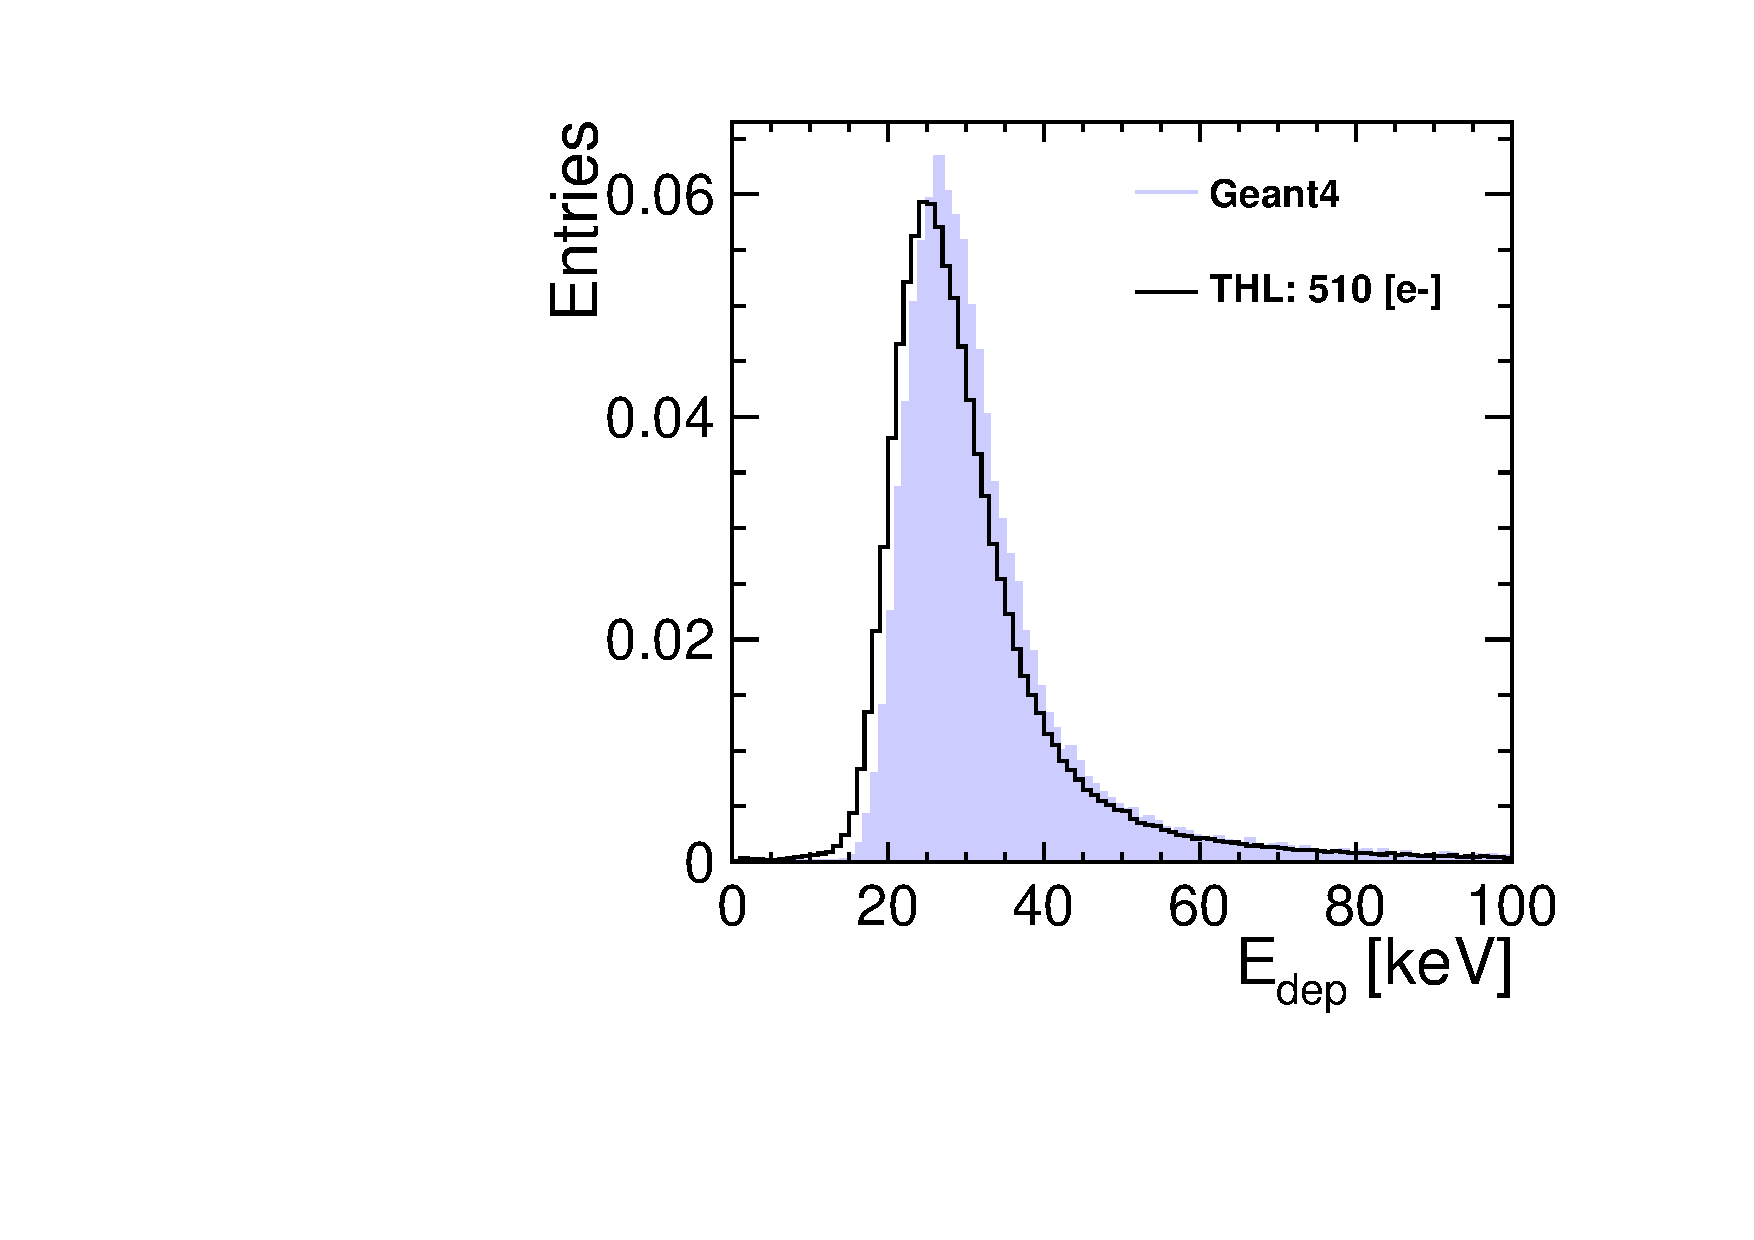
\includegraphics[width=\textwidth]{./figures/Calibration/Edep_G4_W0005_E02.pdf}
    \caption{55-GNDGR-100}
  \end{subfigure}\hfill
  \begin{subfigure}[b]{0.33\textwidth}
    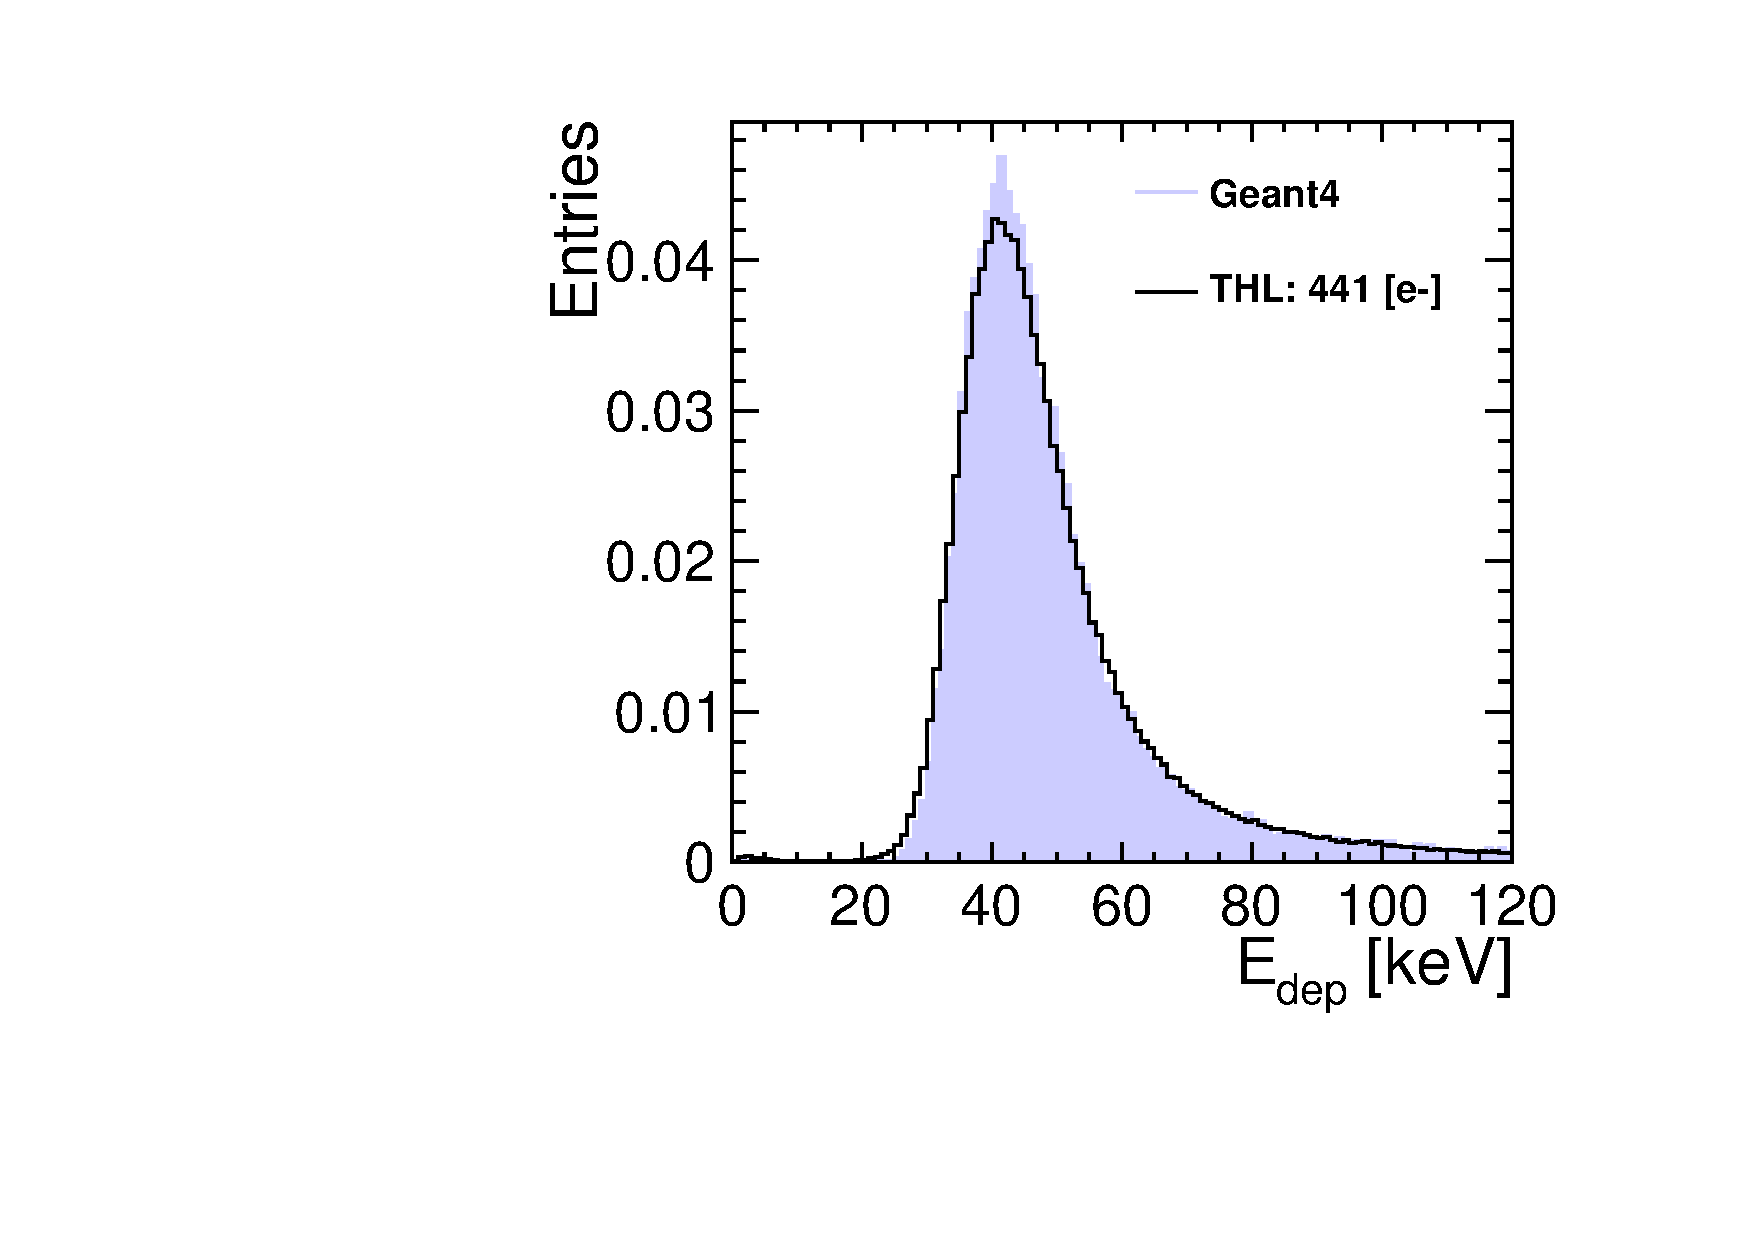
\includegraphics[width=\textwidth]{./figures/Calibration/Edep_G4_W0005_F01.pdf}
    \caption{55-GNDGR-150}
  \end{subfigure}
  \caption{Calibrated energy distribution of test beam data for
    different assemblies. The pixel-by-pixel calibration is applied to
    the data which is obtained using test pulses. \textsc{Geant4}
    energy deposition is obtained using the PAI physics list.}
  \label{sec:testBeamDataCalibrated_vs_G4}
\end{figure}

\cref{sec:testBeamDataCalibrated_TOT} shows the TOT distribution for
one, two, three and four-hit clusters. The MPV of the TOT
distributions for different cluster sizes do not align due to the
non-linear behaviour of the Timepix3, as sharing the same deposited
charge amongst several pixels results in each pixel having a higher
TOT than would be expected from simply scaling the charge. The
calibrated energy distribution aligns for different cluster sizes
since the calibration takes into account the non-linearities of the
chip as shown in \cref{sec:testBeamDataCalibrated_Edep}. For the
$50\,\micron$ thick sensor, the calibrated distributions do not
align. This is due to the low energy deposition in thin sensors
especially for multi-hit clusters where the energy deposition per
pixel is close to the threshold.

\begin{figure}[htbp] \centering
  \begin{subfigure}[b]{0.33\textwidth}
    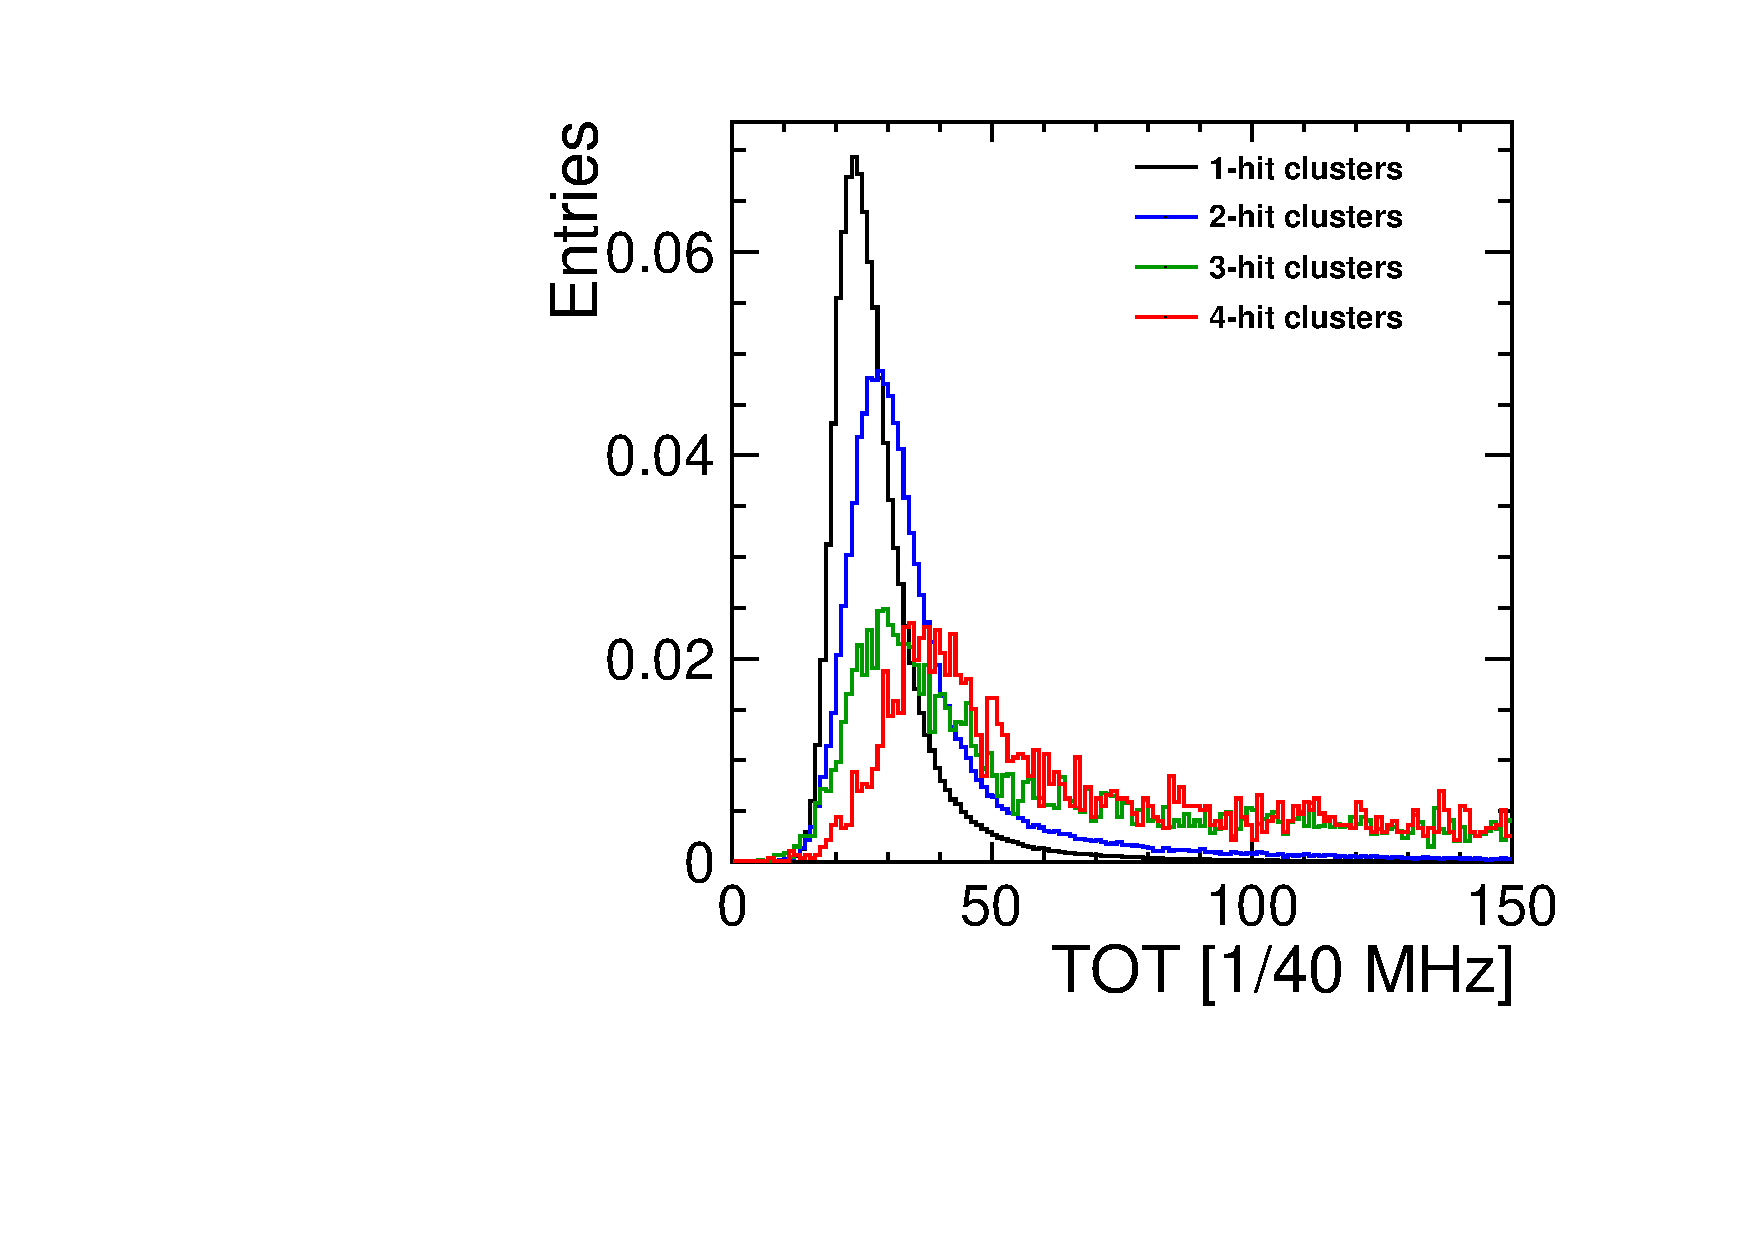
\includegraphics[width=\textwidth]{./figures/Calibration/TOT_Clusters_W0019_G07.pdf}
    \caption{55-GNDGR}
  \end{subfigure} \hfill
  \begin{subfigure}[b]{0.33\textwidth}
    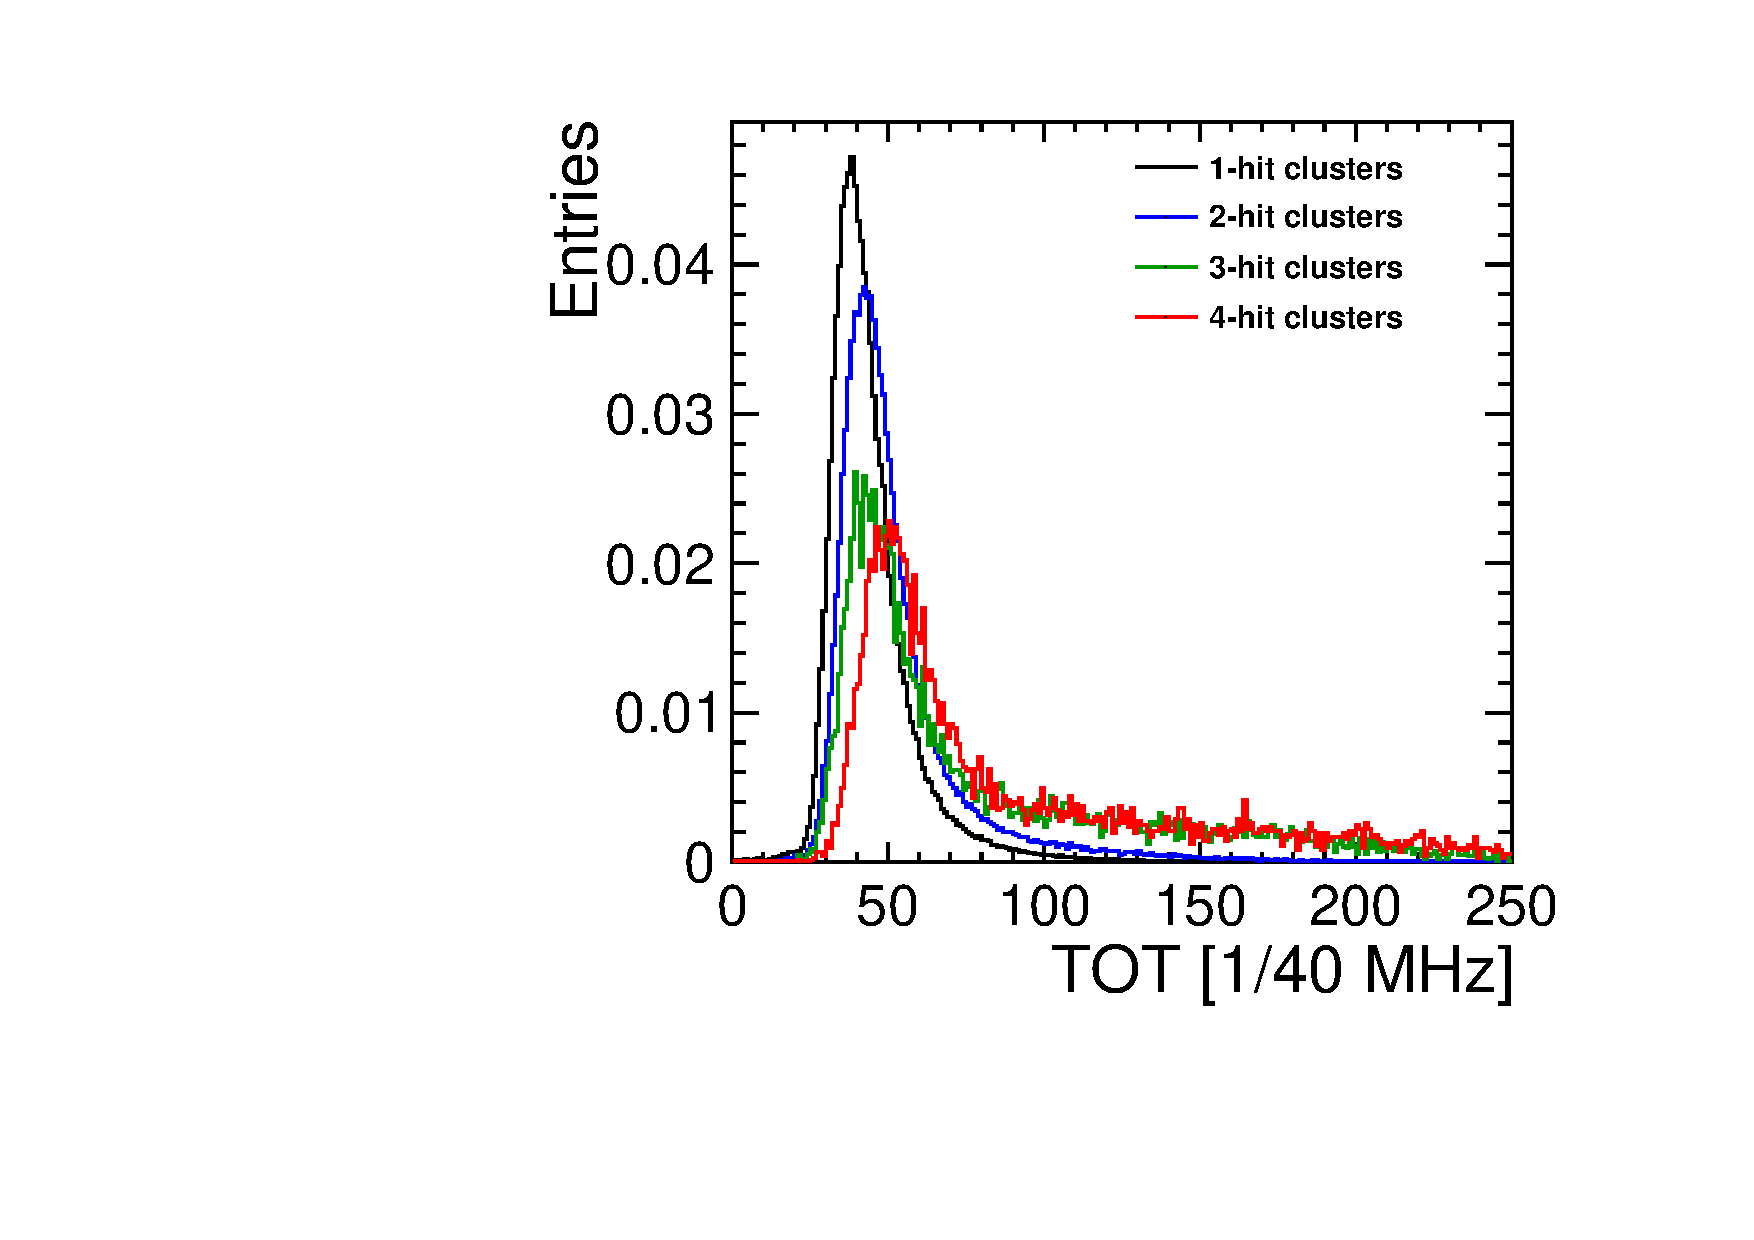
\includegraphics[width=\textwidth]{./figures/Calibration/TOT_Clusters_W0005_E02.pdf}
    \caption{55-GNDGR-100}
  \end{subfigure}\hfill
  \begin{subfigure}[b]{0.33\textwidth}
    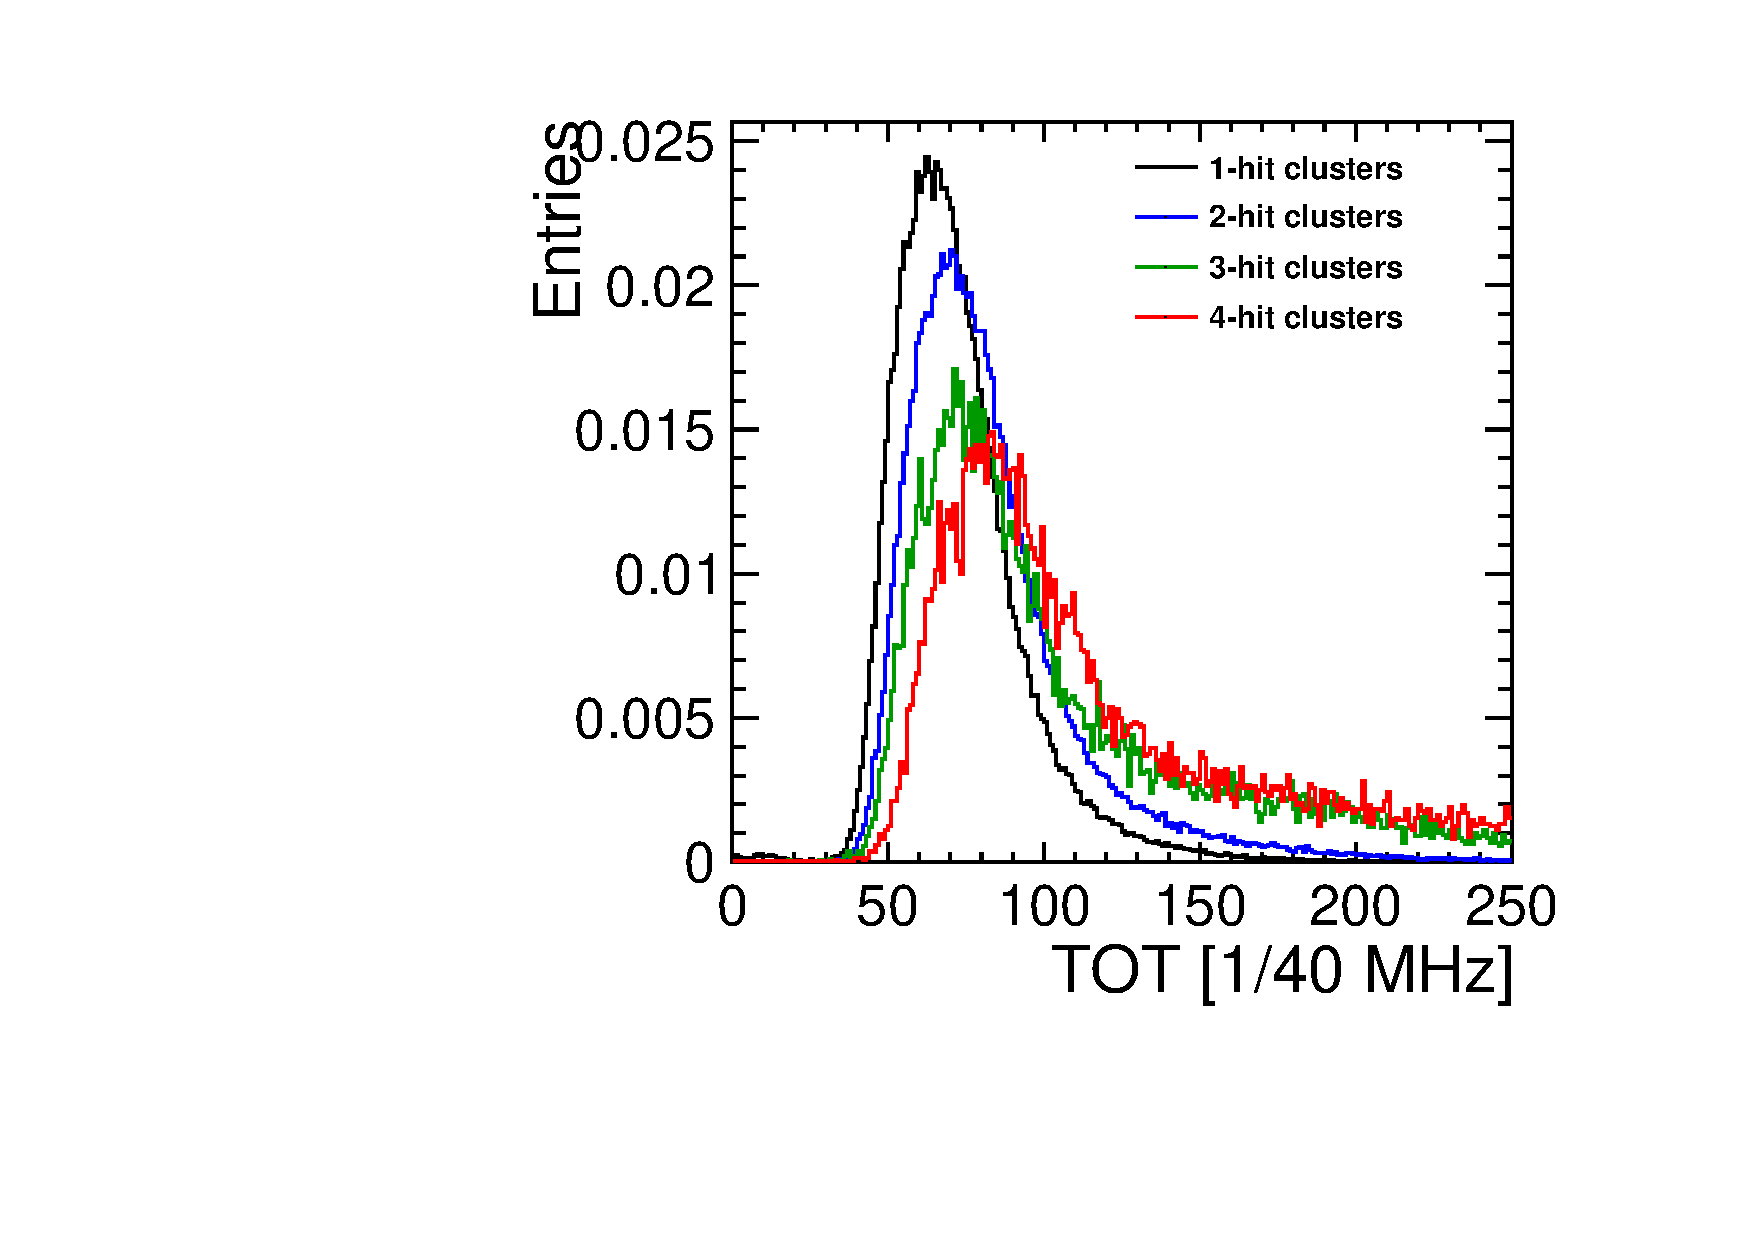
\includegraphics[width=\textwidth]{./figures/Calibration/TOT_Clusters_W0005_F01.pdf}
    \caption{55-GNDGR-150}
  \end{subfigure}
  \caption{TOT distribution for one, two, three and four-hit clusters
    for various assemblies with (a) $50\,\micron$, (b) $100\,\micron$
    and (c) $150\,\micron$ thick planar sensors.}
  \label{sec:testBeamDataCalibrated_TOT}
\end{figure}

\begin{figure}[htbp] \centering
  \begin{subfigure}[b]{0.33\textwidth}
    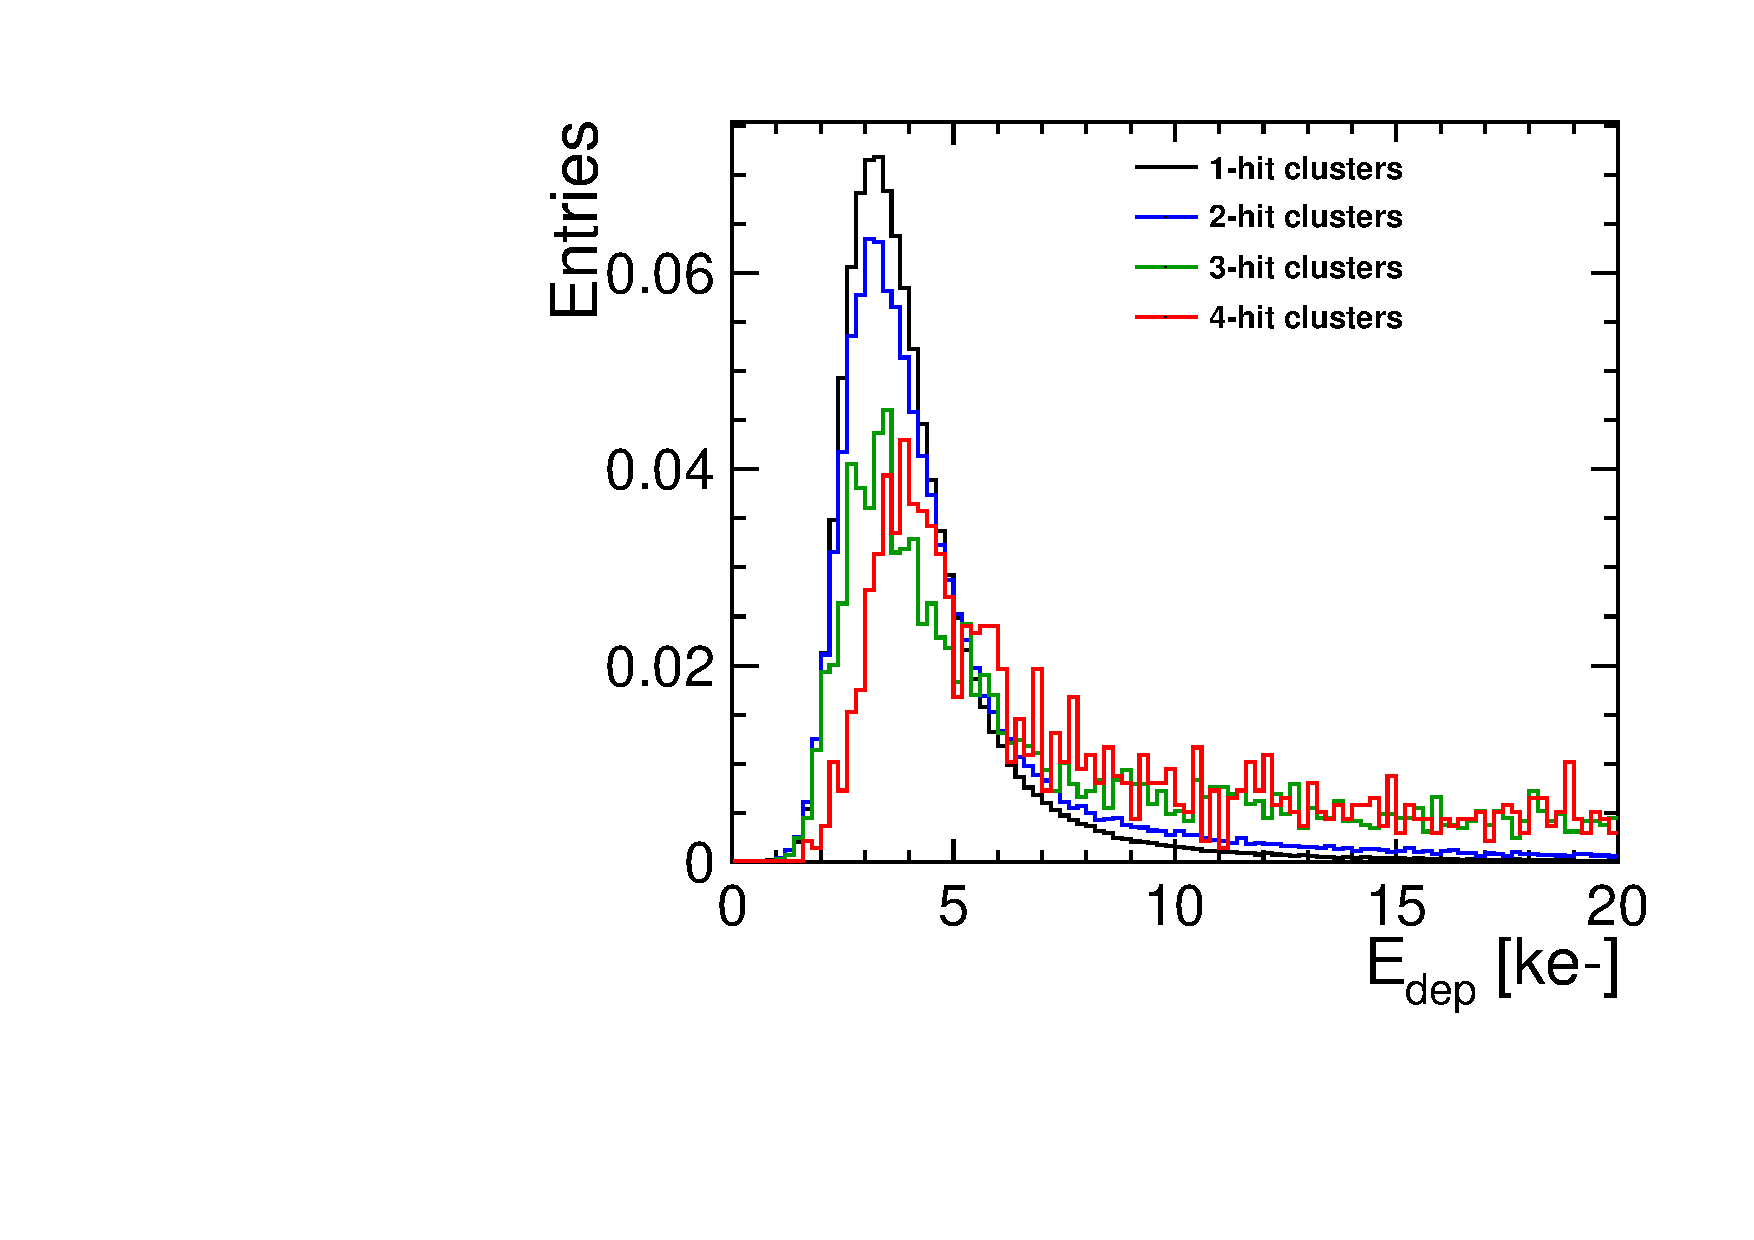
\includegraphics[width=\textwidth]{./figures/Calibration/Edep_Clusters_W0019_G07.pdf}
    \caption{55-GNDGR}
  \end{subfigure} \hfill
  \begin{subfigure}[b]{0.33\textwidth}
    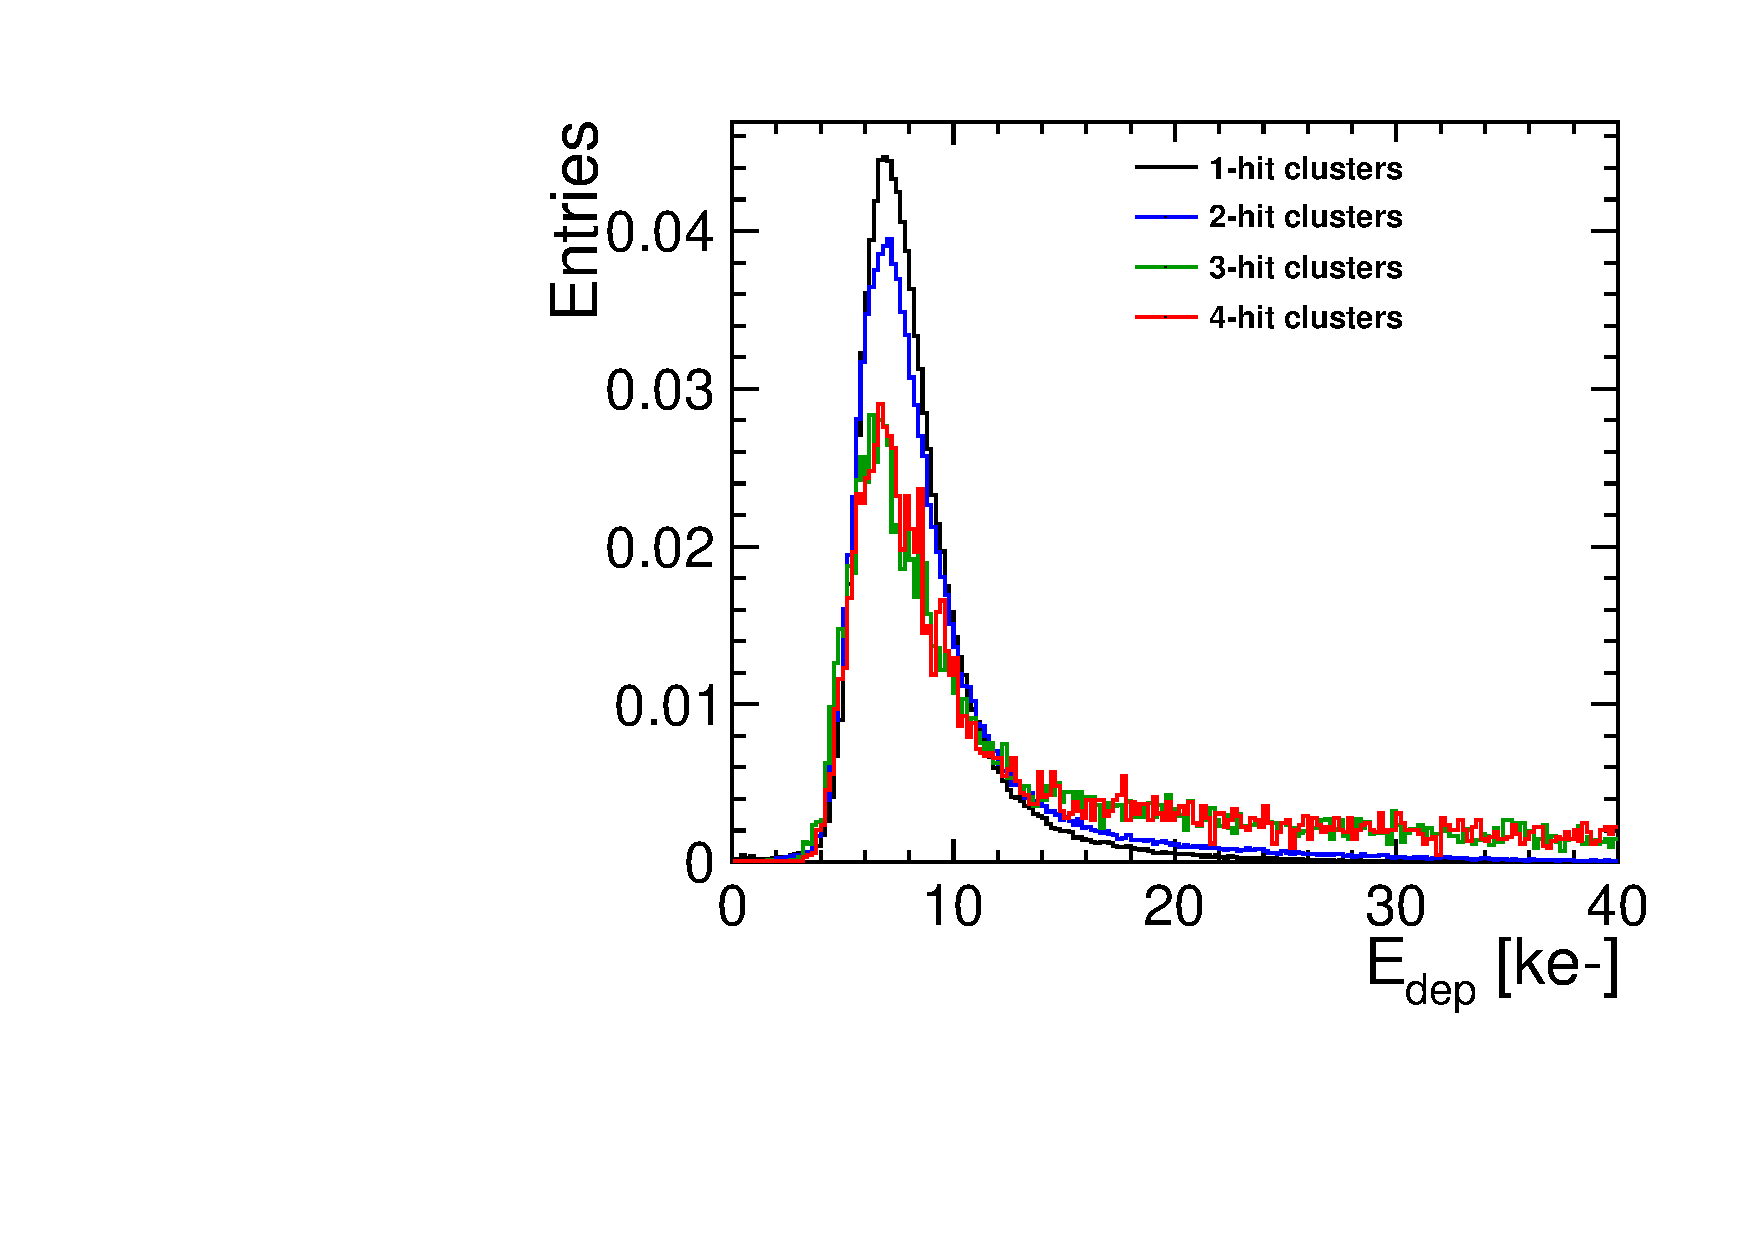
\includegraphics[width=\textwidth]{./figures/Calibration/Edep_Clusters_W0005_E02.pdf}
    \caption{55-GNDGR-100}
  \end{subfigure}\hfill
  \begin{subfigure}[b]{0.33\textwidth}
    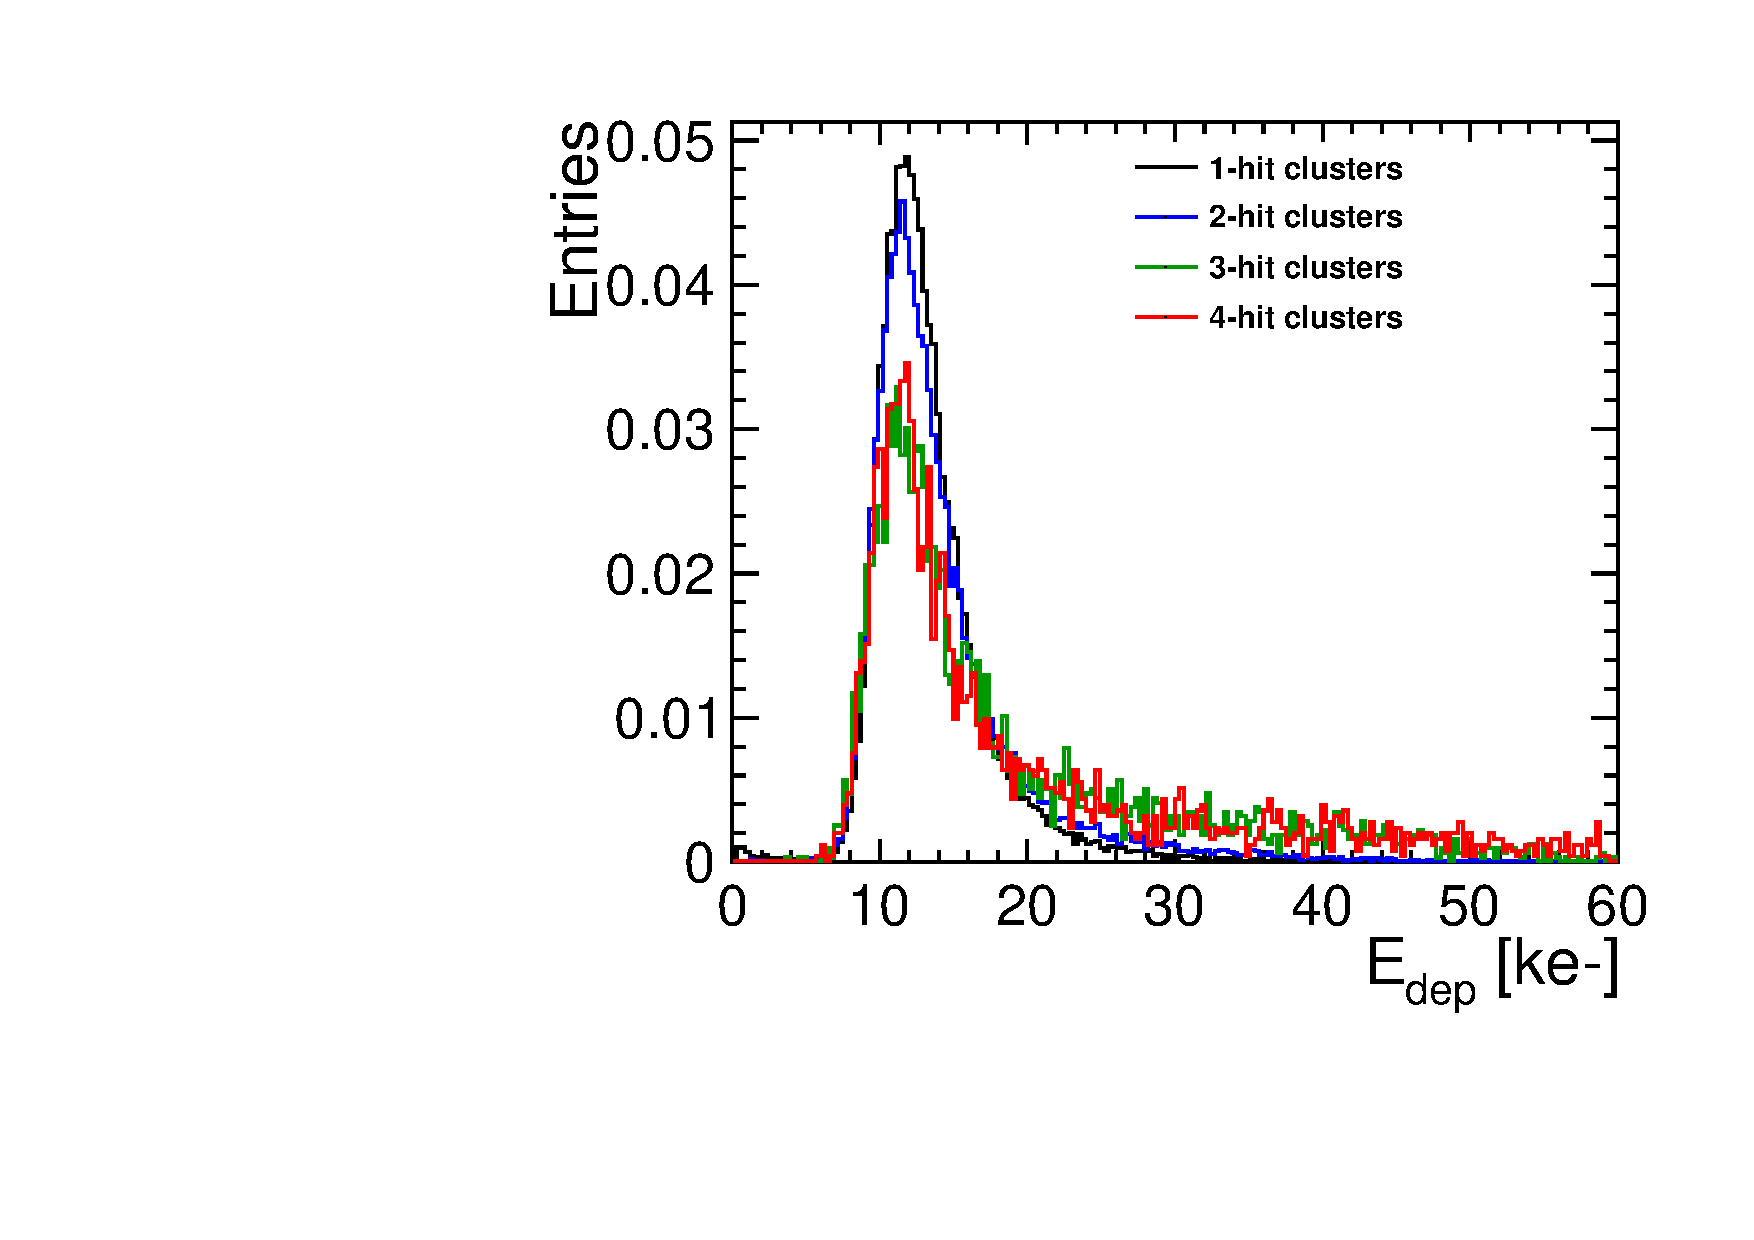
\includegraphics[width=\textwidth]{./figures/Calibration/Edep_Clusters_W0005_F01.pdf}
    \caption{55-GNDGR-150}
  \end{subfigure}
  \caption{Energy deposition distribution for one, two, three and
    four-hit clusters for various assemblies with (a) $50\,\micron$,
    (b) $100\,\micron$ and (c) $150\,\micron$ thick planar sensors.}
  \label{sec:testBeamDataCalibrated_Edep}
\end{figure}

For all the assemblies, the energy deposition in \ev is given in \cref{sec:appendixCalibDataG4}.
%%%%%%%%%%%%%%%%%%%%%%%%%%%%%%%%%%%%%%%%%%%%%%%%%%%%%%%%
%%%%%%%%%%%%%%%%%%%%%%%%%%%%%%%%%%%%%%%%%%%%%%%%%%%%%%%%
%%%%%%%%%%%%%%%%%%%%%%%%%%%%%%%%%%%%%%%%%%%%%%%%%%%%%%%%
% \begin{table}[htbp]
%   \caption{Measured DAC step gain.}
%   \label{tab:DACStep}
%   \centering
%   \begin{tabular}{ c c c }
%     \toprule
%     Assembly & Threshold DAC step [\ev] & Threshold DAC step [\Pem] \\
%     \midrule
%     A06-W0110  & $81\pm0.009$ & $22.475\pm0.025$  \\
%     C04-W0110  & $85\pm0.039$ & $23.544\pm0.011$ \\
%     L04-W0125 &  $86\pm0.022$ & $23.775\pm0.006$ \\
%     B06-W0125  & $86\pm0.120$ & $23.978\pm0.033$ \\
%     \bottomrule
%   \end{tabular}
% \end{table}

% Threshold measurements were not completed for assemblies B07-W0125 and
% D09-W0126. Assembly B07-W0125 did not fully deplete due to a broken
% corner of the sensor. The derivative of the CuXRF S-curve did not form
% a peak as the photon energy was close to the noise level. Assembly
% D09-W0126 was not operating as expected for a $100\,\micron$
% sensor. Therefore the calibration of these assemblies was done without
% threshold measurements.
